\section{Infinite divisibility, necklaces and solved models}\label{ch:rz3}

By Theorem~\ref{rz:thm:w}, $-\varphi'/\varphi$ is the Laplace transform of the canonical function $w=e^{x/4}-P=W-W_0$. Section~\ref{rz:sec:id} proves that $w$ is positive and studies the law whose Laplace transform is $\varphi$. Section~\ref{rz:sec:implications} reads the Vere-Jones weights arithmetically, through the prime number theorem and in a pseudo spectral trace formula, and carries the L\'evy and Thorin representations across the critical strip. Section~\ref{rz:sec:polya} places the solved models in the theory of P\'olya, Cardon, Lee and Yang.

\subsection{Infinite divisibility and the class of \texorpdfstring{$\varphi$}{phi}}\label{rz:sec:id}

Whether $\varphi$ is infinitely divisible is a question about the sign of $w$. A function of the form $\exp(-\int_0^\infty(1-e^{-sx})\,\nu(dx))$, with $\nu\ge0$ and $\int\min(1,x)\,\nu(dx)<\infty$, is the Laplace transform of an infinitely divisible law on $[0,\infty)$ with L\'evy measure $\nu$, and by Theorem~\ref{rz:thm:w} the candidate L\'evy density of $\varphi$ is $w(x)/x$. Recall that $w(0^+)=1$ and $w(x)\sim c/(2\sqrt{\pi x})$ as $x\to\infty$, where $c=-\theta'(0)\approx2.68609$ is the constant of \eqref{rz:eq:c}. The proof of positivity uses the verification of RH to height $50$, classical since Backlund \cite{Backlund} and contained in every later verification \cite{PT21}, the explicit Riemann von Mangoldt bound of Hasanalizade, Shen and Wong \cite{HSW22}, and three interval enclosures, $F(0.004)<-0.111$ for the function $F$ of Lemma~\ref{rz:lem:W0}, $P(0.004)<2\times10^{-13}$ and the tail bound $E(0.004)<0.0011$ for the sum $E$ defined in the proof, computed in outward rounded interval arithmetic by \nolinkurl{verification_reciprocal_zeta/enclosures.py} (enclosures E1 to E3).

\begin{theorem}\label{rz:thm:id}
$w(x)>0$ for every $x>0$. Consequently, unconditionally, $\varphi$ is the Laplace transform of an infinitely divisible probability law on $(0,\infty)$ with zero drift and L\'evy density $w(x)/x$:
\[
\frac{\zeta(\frac12)}{(1-4s)\,\zeta(\frac12+\sqs)}=\exp\Bigl(-\int_0^\infty\bigl(1-e^{-sx}\bigr)\frac{w(x)}{x}\,dx\Bigr),\qquad \Re s>0 .
\]
\end{theorem}

\begin{proof}
Fix $x_1=0.004$.

Small $x$. Each term $x^{-1/2}e^{-(\log n)^2/4x}$ increases in $x$ while $(\log n)^2/4x>\frac12$, which holds for $x\le x_1$ and $n\ge2$. Hence $P(x)\le P(x_1)<2\times10^{-13}$ (enclosure E2: the term $n=2$ in interval arithmetic, and $n\ge3$ through $(\log n)^2/4x_1\ge\frac{\log3}{4x_1}\log n$), and $w(x)=e^{x/4}-P(x)>0$ on $(0,x_1]$.

Large $x$. By Lemma~\ref{rz:lem:W0} and $F(x_1)<0$, for $x\ge x_1$ we have $-W_0(x)\ge|F(x_1)|/(4\sqrt{\pi x})$. Here $F(x_1)<-0.111$ by enclosure E1: an upper Riemann sum of interval suprema of the integrand $e^{-u/4}(1-e^{-u^2/16x_1})/(1-e^{-u})$ of Lemma~\ref{rz:lem:W0} on $[10^{-4},200]$, with the integrand at most $u(1+u)/16x_1$ on $[0,10^{-4}]$ and at most $e^{-u/4}/(1-e^{-200})$ beyond $200$, and $2\theta'(0)=-\gamma_E-\frac\pi2-3\log2-\log\pi$. In $W$ the zeros with $0<\gamma\le50$ lie on the line \cite{Backlund} and contribute $e^{-x\gamma^2}>0$. Any other zero has $\gamma>50$ and contributes at most $e^{-x(\gamma^2-1/4)}$ in modulus. The explicit Riemann von Mangoldt formula $|N(T)-\frac T{2\pi}\log\frac T{2\pi e}-\frac78|\le E(T)$ for $T\ge e$, with $E(T)=2.5167+\frac1{50T}$ for $T\le X_0=30\,610\,046\,000$ and $E(T)=0.1095\log T+0.2042\log\log T+3.0305+\frac1{50T}<0.3\log T$ for $T>X_0$ \cite[(1.7), (2.7) and Corollary~1.4]{HSW22}, gives $N(t+1)-N(t)\le2\log(t+1)$ for $t\ge50$: the main term grows by at most $\frac1{2\pi}\log\frac{t+1}{2\pi}$, and while $t+1\le X_0$ the two error terms add at most $5.0334+\frac1{25t}$, together less than $5.37$ at $t=50$ against $2\log51=7.86$, with a gap that widens as $t$ grows, since its derivative exceeds $(2-\frac1{2\pi})/(t+1)$; for $t+1>X_0$ the error terms add at most $0.6\log(t+1)$, and $\frac1{2\pi}+0.6<2$. So all such zeros together contribute at most
\[
E(x)=\sum_{j\ge0}2\log(51+j)\,e^{-x((50+j)^2-\frac14)} .
\]
Enclosure E3 gives $E(x_1)<0.0011$, against $|F(x_1)|/(4\sqrt{\pi x_1})>0.247$. Since $(50+j)^2-\frac14>1/(2x_1)$ for every $j$, $\sqrt x\,E(x)$ decreases on $[x_1,\infty)$, so $E(x)<|F(x_1)|/(4\sqrt{\pi x})\le-W_0(x)$ for all $x\ge x_1$, and $w=W-W_0>0$ on $[x_1,\infty)$.

Representation. By Theorem~\ref{rz:thm:w}, $-\varphi'/\varphi(s)=\int_0^\infty e^{-sx}w(x)dx$ for $s>\frac14$. Since $w\ge0$, Landau's theorem applies \cite[Chapter~II, Theorem~5b]{Widder41}: if the Laplace transform of a nonnegative function has abscissa of convergence $\sigma_c$, then the transform cannot be continued analytically to a neighbourhood of $\sigma_c$. Here the transform agrees with $-\varphi'/\varphi$ on $(\frac14,\infty)$, and $-\varphi'/\varphi$ is analytic near every point of $(0,\infty)$ by Proposition~\ref{rz:prop:rh}. Hence $\sigma_c\le0$, the integral converges for $\Re s>0$, and equals the continuation of $-\varphi'/\varphi$ there. Integrating over $[a,s]$ for real $0<a<s$ with Tonelli, and letting $a\downarrow0$ with $\varphi(a)\to1$ and monotone convergence, gives the formula for real $s>0$; then $\int\min(1,x)\,w(x)x^{-1}dx<\infty$ because the left side is finite, and analytic continuation gives the formula for $\Re s>0$.
\end{proof}

Theorem~\ref{rz:thm:id} is the main unconditional positive result of Chapter~\ref{chap:rzeta} and of this chapter, and its proof has a wide margin (Figure~\ref{rz:fig:w}). The two halves of the argument overlap: at $x_1=0.004$ the prime sum $P(x_1)$ is below $2\times10^{-13}$ while $-W_0(x_1)$ already exceeds $0.25$, so the positivity of $w$ does not rest on a delicate numerical fact near a single point. The only place where $w$ comes close to a sign change is at infinity, where it decays like $x^{-1/2}$, and there the sign is fixed by $\theta'(0)<0$.

\begin{figure}[htbp]
\centering
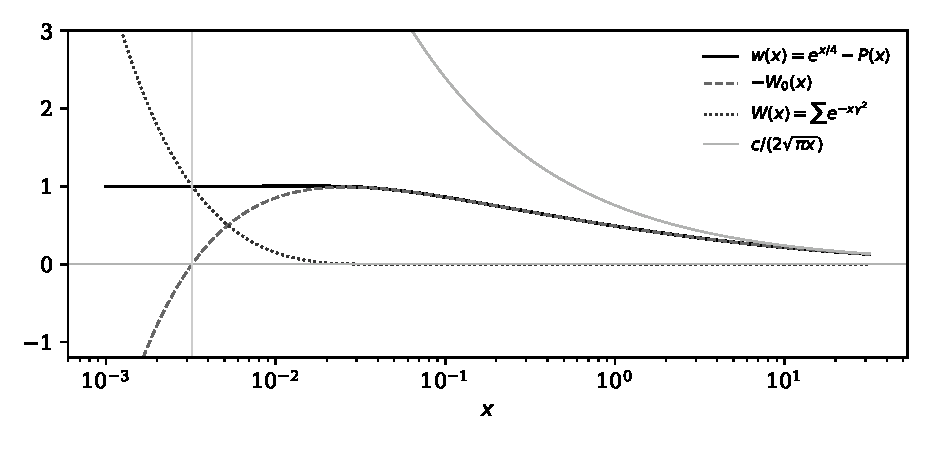
\includegraphics[width=0.9\textwidth]{rzfig/fig_w.pdf}
\caption{The function $w=W-W_0$ on a logarithmic scale, with its two components: the heat trace $W$ over the zeros and the negative smooth part $-W_0$. The vertical line is $x_*\approx0.00322$, where $W_0$ changes sign. To the left, $w$ differs from $e^{x/4}$ by less than $2\times10^{-13}$; to the right, $-W_0>0$, and from $x_1=0.004$ on it dominates any contribution of off line zeros to $W$. The faint curve is the asymptote $c/(2\sqrt{\pi x})$.}
\label{rz:fig:w}
\end{figure}

In arithmetic terms, Theorem~\ref{rz:thm:id} is the Gaussian smoothed Chebyshev bound
\[
\sum_{n\ge2}\frac{\Lambda(n)}{\sqrt n}\,e^{-(\log n)^2/4x}<\sqrt{4\pi x}\;e^{x/4}\qquad(x>0).
\]
The right side is $\int_0^\infty y^{-1/2}e^{-(\log y)^2/4x}\,dy$, the same smoothing applied to $dy$ in place of $d\psi(y)$, where $\psi(y)=\sum_{n\le y}\Lambda(n)$ is Chebyshev's function. The proof uses the zeros only through the ten below height $50$, the explicit bound for $N(T)$ and the monotone archimedean term $F$. To see what the primes alone give, write $\psi(y)=y+\Delta(y)$ and put $I(x)=\frac12e^{x/4}\operatorname{erfc}(\frac{\sqrt x}2)$.

\begin{proposition}\label{rz:prop:bias}
For $x>0$,
\[
w(x)=I(x)-Q_\Delta(x),\qquad Q_\Delta(x)=\frac{1}{\sqrt{4\pi x}}\int_{1^-}^\infty y^{-1/2}e^{-(\log y)^2/4x}\,d\Delta(y),
\]
with $I(x)\sim(\pi x)^{-1/2}$ and $w(x)\sim\frac c2(\pi x)^{-1/2}$ as $x\to\infty$. Hence $Q_\Delta(x)\sim-(\frac c2-1)(\pi x)^{-1/2}$ with $\frac c2-1\approx0.343$. On the other hand, any bound $|\Delta(y)|\le A\sqrt y\log^2y$ for $y\ge2$, including the one that RH implies, yields only $|Q_\Delta(x)|\le A\,(x/2+O(\sqrt x))$ after integration by parts.
\end{proposition}

\begin{proof}
With $d\Delta=d\psi-dy$, the main term is $(4\pi x)^{-1/2}\int_1^\infty y^{-1/2}e^{-(\log y)^2/4x}dy=(4\pi x)^{-1/2}\int_0^\infty e^{u/2-u^2/4x}du=\frac12e^{x/4}(1+\operatorname{erf}\frac{\sqrt x}2)$, and $e^{x/4}$ minus this is $I$. The asymptotics of $w$ are Theorem~\ref{rz:thm:w}. For the bound, integrate by parts and use $\frac{d}{dy}\{y^{-1/2}e^{-(\log y)^2/4x}\}=-y^{-3/2}e^{-(\log y)^2/4x}(\frac12+\frac{\log y}{2x})$ and $\int_0^\infty u^2e^{-u^2/4x}(\frac12+\frac u{2x})du=\frac{\sqrt\pi}2(2\sqrt x)^3\cdot\frac14+4x$; the boundary term at $1^-$ and the range $1\le y<2$ contribute $O(x^{-1/2})$.
\end{proof}

In this Gaussian weighting the error term $\Delta$ of the prime number theorem has a definite negative bias at large $x$, $Q_\Delta(x)\approx-0.343(\pi x)^{-1/2}$, which is $I+W_0$ up to an exponentially small term, and $w>0$ is the statement that $Q_\Delta(x)<I(x)$ for all $x$. Pointwise bounds on $\Delta$, which oscillates with both signs, cannot give this at large $x$: the margin that keeps $w$ positive there is of order $x^{-1/2}$, while a pointwise bound on $\Delta$ controls $Q_\Delta$ only up to order $x$; the function $D(y)=-A\sqrt y\log^2y$, in place of $\Delta$, gives $Q_D(x)=-A\bigl(x/2+2\sqrt{x/\pi}\bigr)$ by the computation in the proof, so the bound of Proposition~\ref{rz:prop:bias} cannot be improved using the size of $\Delta$ alone. Mean square information on $\Delta(y)/\sqrt y$ in the logarithmic scale, of the kind Cram\'er obtained under RH \cite{Cramer}, controls Gaussian smoothed quantities much better, and we make no claim that such information is insufficient. For $x\le0.004$ the primes alone suffice (Theorem~\ref{rz:thm:id}).

\subsubsection{The place of \texorpdfstring{$\varphi$}{phi} in the Bondesson hierarchy}\label{rz:sec:class}

Recall from Section~\ref{sec:ch3:hierarchy} the classes of laws on $[0,\infty)$ defined through the L\'evy density $k(x)/x$: the infinitely divisible laws (ID), the self decomposable laws (SD), for which $k$ is nonincreasing, the Bondesson class (BO), for which $k(x)/x$ is completely monotone, and the GGCs, for which $k$ is completely monotone. They are nested as $\mathrm{GGC}\subset\mathrm{SD}\subset\mathrm{ID}$ and $\mathrm{GGC}\subset\mathrm{BO}\subset\mathrm{ID}$ \cite{Bondesson,SvH}.

\begin{theorem}\label{rz:thm:class}
$\varphi\in\mathrm{ID}$ but $\varphi\notin\mathrm{SD}$, $\varphi\notin\mathrm{BO}$, and $\varphi$ is not a mixture of exponentials. In particular $\varphi$ is not a generalised gamma convolution.
\end{theorem}

\begin{proof}
ID is Theorem~\ref{rz:thm:id}.

SD. A law on $(0,\infty)$ with L\'evy density $k(x)/x$ is self decomposable if and only if $k$ is nonincreasing (Section~\ref{sec:ch3:hierarchy}). If $\varphi$ is not infinitely divisible there is nothing to prove, and if it is then $k=w$ by Theorem~\ref{rz:thm:w}. Now $w=e^{x/4}-P$, and $P$ together with every one of its derivatives vanishes at $0^+$, so $w'(0^+)=\frac14>0$ and $w$ strictly increases at the origin. No numerical value enters, and neither does Theorem~\ref{rz:thm:id}: the case split replaces it.

BO. Membership means that the L\'evy density $w(x)/x$ equals $\int e^{-tx}m(dt)$ for some $m\ge0$. Then $-\varphi'/\varphi(s)=\int_0^\infty xe^{-sx}\int e^{-tx}m(dt)\,dx=\int m(dt)/(s+t)^2$ is analytic on $\cut$, so $\varphi$ has no zeros or poles there and RH follows from Proposition~\ref{rz:prop:rh}. Under RH, Theorem~\ref{rz:thm:w} gives $w(x)=\int e^{-tx}dM(t)$, with $M(t)=N(\sqrt t)-\theta(\sqrt t)/\pi=1+S(\sqrt t)$ as in Theorem~\ref{rz:thm:thorin}, and since $M(0^+)=0$ an integration by parts gives $w(x)/x=\int e^{-tx}M(t)\,dt$. Uniqueness of Laplace transforms gives $M\,dt=m\ge0$, that is $S(\tau)\ge-1$ for almost all $\tau$. But by Selberg's central limit theorem \cite{Selberg46}, $S(\tau)<-1$ for a positive proportion of $\tau\in[T,2T]$ once $T$ is large, so $M<0$ on a set of positive measure. Numerically, for $527.71\le\tau\le527.90$, just below $\gamma_{289}=527.9036\ldots$, ball arithmetic gives $N(\tau)=288$ and $-1.143<S(\tau)<-1.008$, so $M<0$ there, and $S(\gamma_{289}^-)=-1.14548\ldots$ (\nolinkurl{verification_reciprocal_zeta/certify_k9_k2.py}).

Mixtures of exponentials. The law is a mixture of exponentials exactly when it has a completely monotone density, that is when $\varphi$ is a Stieltjes function, which requires $\Im\varphi(-t+i0)$ to have one sign. With $\zeta(\frac12+i\tau)=Z(\tau)e^{-i\theta(\tau)}$ we get $\Im\varphi(-\tau^2+i0)=\zeta(\frac12)\sin\theta(\tau)/\{(1+4\tau^2)Z(\tau)\}$. On $(0,\gamma_1)$, $Z$ has no zero while $\theta$ decreases through $-\pi$ at $\tau_\pi=3.43622\ldots$, so $\sin\theta$ changes sign.

GGC. Since GGC is contained in SD and in BO, either clause excludes it. The exclusion also follows directly, without computation. If $\varphi$ were the transform of a GGC then $-\varphi'/\varphi$ would be a Stieltjes function $a+\int U(dt)/(s+t)$ with $U\ge0$, that is $a+\int_0^\infty e^{-sx}\bigl(\int e^{-tx}U(dt)\bigr)dx$. Comparing with $-\varphi'/\varphi(s)=\int_0^\infty e^{-sx}w(x)\,dx$ of Theorem~\ref{rz:thm:w} on $s>\frac14$, uniqueness of Laplace transforms forces $a=0$ and $w(x)=\int e^{-tx}U(dt)$, completely monotone and in particular nonincreasing, against $w'(0^+)=\frac14>0$.
\end{proof}

The theorem is unconditional. Its ID clause rests on Theorem~\ref{rz:thm:id}, its BO clause on Selberg's central limit theorem for $S$, and its SD clause and the conclusion $\varphi\notin\mathrm{GGC}$ on no computation. Since mixtures of exponentials lie in BO \cite{Bondesson}, the mixture clause also follows from the BO clause, and from $f'(0^+)>0$ in Theorem~\ref{rz:thm:shape}; the direct argument, through the computed value of $\tau_\pi$, is an independent check.

The failures have two causes, and neither involves a zero off the line. Self decomposability and the GGC property fail because of the pole: the factor $1-4s$ that removes it puts $e^{x/4}$ into $w$, so the canonical function increases near the origin. This is a property of the normalisation, and Proposition~\ref{rz:prop:onlyhalf} shows the same on every line of the strip. The Bondesson property fails because the negative Thorin density of the gamma factor meets the fluctuations of the zeros about their smooth count, measured by $S$, which has large negative excursions: the first zero with $S(\gamma^-)<-1$ is $\gamma_{127}=282.4651$, where $S(\gamma_{127}^-)=-1.0063$, and the most negative value among the first $460$ zeros is at $\gamma_{289}$ (the seven such zeros are listed after Theorem~\ref{rz:thm:kappaexact}, and these values of $S$ are enclosed in ball arithmetic by the program cited in the proof). This failure would occur even if RH were true, and since $S$ is unbounded below, by Selberg and Tsang \cite{Selberg46,Tsang}, it recurs infinitely often. Both causes disappear for the completed function $R$, which is infinitely divisible and self decomposable with no hypothesis, by Theorem~\ref{thm:ch12:idsd} \cite[Theorem A]{P26}. What Theorem~\ref{rz:thm:id} adds there is the floor of Theorem~\ref{rz:thm:floor}: the canonical function of $e^{-c\sqs}R(s)$ splits into the arithmetic part $w$ and a completely monotone archimedean part (Section~\ref{ch:rz2}).

\subsubsection{The density of the law}

Let $X_\varphi$ be, as in Section~\ref{ch:rz2}, a random variable with $\E e^{-sX_\varphi}=\varphi(s)$. Differentiating the representation of Theorem~\ref{rz:thm:id} gives $-\varphi'(s)=\varphi(s)\int_0^\infty e^{-sx}w(x)\,dx$, which says that the measure $x\Pr(X_\varphi\in dx)$ is the convolution of the law of $X_\varphi$ with $w(x)\,dx$. Since $\varphi(s)\to0$ as $s\to\infty$, the law has no atom at $0$, so it is absolutely continuous, and its density $f$ satisfies Steutel's equation \cite[Proposition~III.4.16]{SvH}
\begin{equation}\label{rz:eq:steutel}
x\,f(x)=\int_0^xf(x-y)\,w(y)\,dy,\qquad x>0 .
\end{equation}
The right side is continuous in $x$ by dominated convergence, since $f$ is integrable and $w$ is bounded and continuous on $[0,\infty)$, so $f$ may be taken continuous on $(0,\infty)$. Near the origin, $w(y)=1+O(y)$ gives $f(x)=\bar f(x)(1+O(x))$ with $\bar f(x)=x^{-1}\int_0^xf$, and $\bar f(x)>0$ for every $x>0$, since otherwise $s\varphi(s)\to0$, whereas $s\varphi(s)\to-\zeta(\frac12)/4>0$. As $\bar f'=(f-\bar f)/x$, this gives $(\log\bar f)'=O(1)$ near $0$, so $\bar f$ and $f$ have a common positive limit $f(0^+)$, and dominated convergence in $s\varphi(s)=\int_0^\infty e^{-y}f(y/s)\,dy$, $f$ being bounded, gives $f(0^+)=\lim_{s\to\infty}s\varphi(s)=-\zeta(\frac12)/4\approx0.36509$.

At infinity the same equation gives $f(x)\sim w(x)/x\sim\frac{c}{2\sqrt\pi}x^{-3/2}\approx0.75773\,x^{-3/2}$, in three steps. First, $xf(x)\le\sup w$. Second, split the integral in \eqref{rz:eq:steutel}, written as $\int_0^xf(u)w(x-u)\,du$, at $u=x/2$: the part $u\le x/2$ is at most $\sup_{y\ge x/2}w(y)=O(x^{-1/2})$, and the part $u\ge x/2$ is at most $\sup_{[x/2,x]}f\cdot\int_0^{x/2}w=O(x^{-1})\,O(x^{1/2})$, so $f(x)=O(x^{-3/2})$. Third, with this bound the part $u\ge x/2$ is $O(x^{-1})=o(w(x))$, while the part $u\le x/2$ is $w(x)(1+o(1))$ by dominated convergence, since $w(x-u)/w(x)\to1$ for fixed $u$ and stays below $2$ for $u\le x/2$ and large $x$. Hence $xf(x)=w(x)(1+o(1))$. It follows that $\Pr(X_\varphi>x)\sim\frac{c}{\sqrt\pi}x^{-1/2}$ and $\E X_\varphi=\infty$, and since $\varphi(s)=1-c\sqs+O(s)$ gives $\varphi(s/n^2)^n\to e^{-c\sqs}$, the variable $X_\varphi$ lies in the domain of attraction of the positive stable law of index $\frac12$ that generates the building blocks \eqref{rz:eq:levy}. Figure~\ref{rz:fig:f} shows $f$ on logarithmic axes, recovered from $\varphi$ by numerical Laplace inversion; the value at $0^+$ and the $x^{-3/2}$ decay are its two straight portions.

\begin{figure}[htbp]
\centering
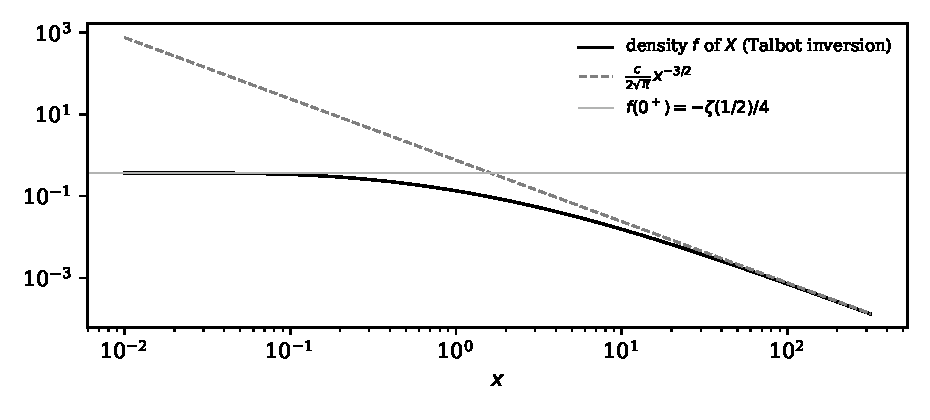
\includegraphics[width=0.9\textwidth]{rzfig/fig_f.pdf}
\caption{The density $f$ of the infinitely divisible law $X_\varphi$ with $\E e^{-sX_\varphi}=\varphi(s)$, computed by Talbot inversion, on logarithmic axes. It starts at $f(0^+)=-\zeta(\frac12)/4$ and decays like $\frac{c}{2\sqrt\pi}x^{-3/2}$. In the legend, $X$ is $X_\varphi$.}
\label{rz:fig:f}
\end{figure}

\begin{theorem}\label{rz:thm:shape}
$f(0^+)=-\zeta(\frac12)/4$ and $f'(0^+)=f(0^+)\,w'(0^+)=-\zeta(\frac12)/16\approx0.09127>0$. In particular $f$ is not monotone, so $X_\varphi$ is not a mixture of uniform laws on intervals $[0,a]$, and $f$ is not log convex and not completely monotone.
\end{theorem}

\begin{proof}
The value of $f(0^+)$ was found after \eqref{rz:eq:steutel}. Since $P$ and all its derivatives vanish at $0^+$, $w$ is continuously differentiable on $[0,\infty)$ with $w(0^+)=1$ and $w'(0^+)=\frac14$. Write \eqref{rz:eq:steutel} as $xf(x)=\int_0^xf(u)\,w(x-u)\,du$. Since $f$ is continuous on $(0,\infty)$ and bounded near $0$, the right side is differentiable, with derivative $f(x)w(0^+)+\int_0^xf(u)w'(x-u)\,du$, so $f$ is differentiable on $(0,\infty)$ and
\[
f'(x)=\frac1x\int_0^xf(u)\,w'(x-u)\,du\longrightarrow f(0^+)\,w'(0^+)\qquad(x\downarrow0),
\]
because $f$ and $w'$ are continuous at $0$. A nonincreasing density is required for a mixture of uniforms by Khintchine's theorem, and log convex or completely monotone densities are nonincreasing.
\end{proof}

\begin{proposition}\label{rz:thm:unimod}
$w'>0$ on $(0,0.004]$ and $w'<0$ on $[4.52,\infty)$. On $[0.004,4.6]$ a grid evaluation of $w'$ (computed, not proved) finds exactly one sign change, at $x_m=0.015851\ldots$, where $w(x_m)=1.003409\ldots$.
\end{proposition}

\begin{proof}
On $(0,0.004]$, $w'=\frac14e^{x/4}-P'(x)$ and $0\le P'(x)\le P'(0.004)<2\times10^{-9}$, since each prime term of $P'$ increases in $x$ there. For $x\ge0.004$ write $w'=W'-W_0'$. The zeros on the line contribute $-\sum\gamma^2e^{-x\gamma^2}<0$ to $W'$. Every zero below height $3\times10^{12}$ lies on the line \cite{PT21}, so an off line zero contributes at most $(\gamma^2+\frac14)e^{-x(\gamma^2-1/4)}$ with $\gamma>3\times10^{12}$. With $N(t+1)-N(t)\le2\log(t+1)$ from the proof of Theorem~\ref{rz:thm:id}, these contributions together are less than $e^{-10^{22}}\gamma_1^2e^{-x\gamma_1^2}$ for $x\ge0.004$, a negligible fraction of the term of $\gamma_1$; hence $W'<0$. By Proposition~\ref{rz:prop:bernstein}, with $\nu(dy)=2\sum_{k\ge0}e^{-(2k+\frac12)y}\,dy$ the measure defined there,
\begin{gather*}
-W_0'(x)=\frac{D(x)}{4\sqrt\pi\,x^{3/2}},\qquad D(x)=\theta'(0)+\frac12\int_0^\infty g\Bigl(\frac{y^2}{4x}\Bigr)\nu(dy),\\
g(u)=1-(1-2u)e^{-u}.
\end{gather*}
Since $g(0)=0$, $g'(0)=3$, $g$ is concave on $[0,\frac52]$ and $g\le1+2e^{-3/2}<3u$ beyond, $g(u)\le3u$ for all $u\ge0$. With $\int y^2\nu(dy)=4\sum_{k\ge0}(2k+\frac12)^{-3}<32.34$ this gives $D(x)\le\theta'(0)+12.13/x<0$ for $x\ge4.52$, and then both parts of $w'$ are negative.
\end{proof}

The computed statement comes from an evaluation of $w'$ on $[0.004,4.6]$ from the first 300 zeros and the integral for $W_0'$, on a grid of spacing $10^{-4}$ up to $0.05$ and $5\times10^{-3}$ beyond. On this grid $w'$ has exactly one sign change, at $0.01585$, and $|w'|\ge0.024$ at grid points more than $0.002$ from it; the prime and zero evaluations of $w'$ agree to $10^{-11}$ at $x=0.01$. Between two grid points $h$ apart at which $w'$ has one sign and $|w'|\ge0.024$, a further pair of sign changes would need $|w''|\ge2\cdot0.024/h$, that is $|w''|\ge9.6$ where the spacing is $5\times10^{-3}$ and $|w''|\ge480$ where it is $10^{-4}$. An upper bound on $|w''|$ below these values, which is not derived here, would exclude further sign changes away from $x_m$. Within $0.002$ of $x_m$ the grid gives no such margin, and a proof would also need $w''<0$ there, or a bound on $w'''$. Together these would turn the computation into a proof that $w$ is unimodal.

Numerically $f$ is unimodal as well: it rises from $0.365089$ to its maximum $0.366883$ at the mode $x=0.024046$ and then decreases to $0$ like $0.75773\,x^{-3/2}$, so its mode lies to the right of the maximum of $w$. Talbot and de Hoog inversion agree to twelve digits at every point used. Unimodality of $f$ remains open (Section~\ref{rz:sec:open}). Since $X_\varphi$ is infinitely divisible but not self decomposable, Yamazato's theorem that every self decomposable law is unimodal \cite{Yamazato78}, \cite[Theorem~53.1]{Sato99} does not apply, and the rise of $f$ near $0$ (Theorem~\ref{rz:thm:shape}) shows that the question is not trivial. Section~\ref{ch:sato} applies the theorem to the law of $X_R$, which is self decomposable, and to the shifted clocks $T_\alpha$ of Theorem~\ref{thm:poisson} with $\alpha\ge1$ (Corollary~\ref{sb:cor:unimodal}).

\subsubsection{Closure operations and the harmonic mean}

GGC is closed under independent sums and weak limits, and, by a theorem of Bondesson \cite{Bond2015}, under independent products. Any variable assembled from GGC variables by these operations is GGC, so Theorem~\ref{rz:thm:class} gives at once the following.

\begin{corollary}\label{rz:cor:hm}
$X_\varphi$ is not a sum or a product of independent GGC variables, nor a weak limit of such.
\end{corollary}

The reciprocal in $\varphi$ suggests a fourth operation, the harmonic mean. Closure under it would be the statement
\[
\mathrm{(H)}\qquad\text{if $V_1$ and $V_2$ are independent GGC variables, then so is $2V_1V_2/(V_1+V_2)$,}
\]
which would have widened Corollary~\ref{rz:cor:hm}; it is false.

\begin{proposition}\label{rz:prop:hmfalse}
(H) is false. If $E_1$ and $E_2$ are independent standard exponentials, then $H=2E_1E_2/(E_1+E_2)$ has density
\[
f_H(h)=e^{-h}\int_0^\infty\Bigl(1+\frac h{2u}\Bigr)e^{-u-h^2/4u}\,du,\qquad h>0,
\]
and $H$ is not a GGC.
\end{proposition}

\begin{proof}
For $h>0$, $2E_1E_2>h(E_1+E_2)$ holds if and only if $E_1,E_2>\frac h2$ and $(2E_1-h)(2E_2-h)>h^2$: both factors cannot be negative, since $E_1,E_2<\frac h2$ forces $|2E_1-h|,|2E_2-h|<h$. Substituting $E_1=\frac h2+u$, $E_2=\frac h2+v$ gives
\[
\Pr(H>h)=e^{-h}\iint_{uv>h^2/4}e^{-u-v}\,du\,dv=e^{-h}\int_0^\infty e^{-u-h^2/4u}\,du,
\]
so the survival function is $e^{-h}$ times a Laplace type integral. Differentiating under the integral, which is justified by the bound $\frac h{2u}e^{-u-h^2/4u}\le u^{-1/2}e^{-u}\sup_{y>0}ye^{-y^2}$, locally uniform in $h$, gives $f_H$. In terms of the modified Bessel functions of the second kind the two integrals are $h\,\mathrm{K}_1(h)$ and $h\{\mathrm{K}_0(h)+\mathrm{K}_1(h)\}$, by $\int_0^\infty u^{-\nu-1}e^{-u-h^2/4u}\,du=2(h/2)^{-\nu}\mathrm{K}_\nu(h)$ \cite[(10.32.10)]{DLMF}. Splitting the integral at $u=h$ shows that $f_H$ is bounded with $f_H(0^+)=1$.

Suppose $H$ were a GGC with drift $a$ and Thorin measure $U$ of total mass $\beta$. Since $f_H>0$ on $(0,\infty)$ and a GGC satisfies $H\ge a$ almost surely, $a=0$. Since $f_H$ is bounded, $s\,\E e^{-sH}=\int_0^\infty e^{-y}f_H(y/s)\,dy\to f_H(0^+)=1$, so $-\log\E e^{-sH}=\log s+o(1)$, while Fatou applied to $\int\log(1+s/t)\,U(dt)$ gives $\liminf_{s\to\infty}(-\log\E e^{-sH})/\log s\ge\beta$. Hence $\beta\le1$.

Now let $V$ be any GGC with zero drift and $\beta\le1$, and $\mathcal L(s)=\E e^{-sV}$. For $\Im s>0$ each $1+s/t$ lies in the upper half plane, so $\Im\log\mathcal L(s)=-\int\arg(1+s/t)\,U(dt)\in[-\pi\beta,0)\subseteq[-\pi,0)$, and $\mathcal L>0$ on $(0,\infty)$: $\mathcal L$ is a Stieltjes function \cite[Corollary~7.4]{boSSV}. In its representation $\mathcal L(s)=b_0+b_1/s+\int(s+r)^{-1}m(dr)$ \cite[Definition~2.1]{boSSV} we have $b_0=\lim_{s\to\infty}\mathcal L(s)=0$ and $b_1=0$, since $\mathcal L(0^+)=1$. So $\mathcal L(s)=\int_0^\infty e^{-sx}\bigl(\int e^{-rx}m(dr)\bigr)dx$ and the density of $V$ is $\int e^{-rx}m(dr)$, completely monotone and in particular nonincreasing.

But $f_H$ is not nonincreasing: $f_H(h)-1\sim h\log(1/h)$ as $h\downarrow0$, and $f_H$ attains $1.11125$ at $h=0.09765$ against $f_H(0^+)=1$. So $H$ is not a GGC.
\end{proof}

There is also a structural obstruction. The factorisation of $\varphi$ into $R$ and the gamma factor is a factorisation of Laplace transforms, that is a convolution of laws, while (H) acts on the variables themselves. The gamma factor is not a Laplace transform at all, since it tends to infinity with $s$, and \eqref{rz:eq:decon} shows that it enters only through deconvolution by stable laws. The one place where (H) could have acted is the positive part: $R$ is GGC if and only if RH holds, so an unconditional representation $X_R\overset{d}{=}2V_1V_2/(V_1+V_2)$ with $V_1,V_2$ independent GGC variables built from the primes and the gamma factor would have proved RH under (H). Proposition~\ref{rz:prop:hmfalse} removes the implication, and we know of no candidate representation. The kernel of the Vere-Jones identity is itself a harmonic mean of functions, $\sech(\lambda\sqs)=2/(e^{\lambda\sqs}+e^{-\lambda\sqs})$, of the stable transform $e^{-\lambda\sqs}$ and its reciprocal, which is not a transform; and each zero factor satisfies $1+u^2/\gamma^2=2/\{(1+iu/\gamma)^{-1}+(1-iu/\gamma)^{-1}\}$. Neither is a harmonic mean of independent variables, so neither brings (H) into play.

\subsection{The Vere-Jones weights and the L\'evy representation across the strip}\label{rz:sec:implications}

The weights $B_N$ of the logarithmic Vere-Jones representation (Theorem~\ref{rz:thm:saw}) are necklace polynomials evaluated at $p^{-1/2}$, and prime by prime the representation is a deformation of Euler's binary product. In its cyclotomic form the normalisation at the edge of the pole rests on the prime number theorem, and its heat trace form is a trace formula in which the zeros of $\zeta$ appear as a signed superposition of arithmetic progressions. The same weights, evaluated at $p^{-\sigma}$, carry the L\'evy representation to every vertical line of the critical strip, and on these lines the completed function $R_\sigma$ has the Thorin property exactly to the right of all zeros. Throughout this subsection $\sigma$ is the real part of the argument $z$ of $\zeta$.

\subsubsection{Necklace polynomials and the sign rule}

Let $M_k(q)=\frac1k\sum_{d\mid k}\mu(k/d)\,q^d$ be the necklace polynomial \cite{MR}, which for integer $q$ counts aperiodic necklaces of length $k$ in $q$ colours.

\begin{theorem}\label{rz:thm:necklace}
$B_N=0$ unless $N=p^n$ is a prime power, and then
\[
B_{p^n}=b_n\bigl(p^{-1/2}\bigr),\qquad b_n(q)=\sum_{i\ge0,\ 2^i\mid n}M_{n/2^i}(q).
\]
Equivalently, for $|y|<1$ and $0<q\le1$,
\begin{equation}\label{rz:eq:binarycyclo}
\frac1{1-qy}=\prod_{n\ge1}\bigl(1+y^n\bigr)^{b_n(q)},
\end{equation}
so that $\zeta(\frac12+u)=\prod_p\prod_n(1+p^{-nu})^{b_n(p^{-1/2})}$ for $\Re u>\frac12$. At $q=1$, $b_n(1)=1$ if $n$ is a power of $2$ and $0$ otherwise, and \eqref{rz:eq:binarycyclo} becomes Euler's binary identity $\frac1{1-y}=\prod_{j\ge0}(1+y^{2^j})$.
\end{theorem}

\begin{proof}
From the definition of $B_N$ in Theorem~\ref{rz:thm:saw}, $B_{p^n}=\sum_{jm=n}d_m\,a_{p^j}$ with $a_{p^j}=q^j/j$. Proposition~\ref{rz:prop:eta} gives $y^j=\sum_md_m\log(1+y^{mj})$; multiplying by $q^j/j$ and summing over $j$ gives $\sum_nb_n(q)\log(1+y^n)=\sum_jq^jy^j/j=-\log(1-qy)$, which is \eqref{rz:eq:binarycyclo}. The cyclotomic identity $\frac1{1-qy}=\prod_k(1-y^k)^{-M_k(q)}$ and $\log(1+y^n)=\log(1-y^{2n})-\log(1-y^n)$ give, comparing coefficients of $\log(1-y^n)$, the recursion $b_n=M_n+b_{n/2}$ for even $n$ and $b_n=M_n$ for odd $n$, whose solution is the stated sum. At $q=1$, $M_k(1)=\frac1k\sum_{d\mid k}\mu(k/d)=\delta_{k,1}$.
\end{proof}

The identity \eqref{rz:eq:binarycyclo} is a $2$ adic variant of the cyclotomic identity of Metropolis and Rota \cite{MR}; we have not found it stated in this form, but it may well be known in the combinatorics of necklaces. Its exponents include $b_2=\frac{q^2+q}2$, $b_3=\frac{q^3-q}3$, $b_4=\frac{q^4}4+\frac{q^2}4+\frac q2$, $b_6=\frac{q^6+q^3-q^2-q}6$, which give $B_4$, $B_8$ and $B_9$ of Theorem~\ref{rz:thm:saw} and, at $p=2$, $B_{16}$ and $B_{64}$, and numerically both sides agree to $25$ digits at $q=2^{-1/2}$, $y=\frac12$. The identity factors a geometric series into products of $1+y^n$, and applied prime by prime it factors the zeta function into solved models. So the Vere-Jones factorisation of each Euler factor is a deformation of Euler's binary product: on the line $\sigma=0$, where $q=p^{-\sigma}=1$, every exponent is $0$ or $1$ and every factor $1+p^{-2^ju}$ is a solved model with unit multiplicity, while on the critical line the exponents become necklace polynomials evaluated at $p^{-1/2}$.

\begin{proposition}\label{rz:prop:signs}
For every prime $p$, with $q=p^{-1/2}$: $b_{2^a}(q)>0$ for all $a\ge1$, and for odd $n>1$, $b_n(q)\ne0$ and the sign of $b_n(q)$ is $(-1)^{\omega(n)}$, where $\omega(n)$ is the number of distinct prime factors of $n$.
\end{proposition}

\begin{proof}
For $n=2^a$, $b_n=q+\sum_{j=1}^a\frac{q^{2^j}-q^{2^{j-1}}}{2^j}=\frac q2+\frac{q^2}4+\cdots+\frac{q^{2^{a-1}}}{2^a}+\frac{q^{2^a}}{2^a}>0$. For odd $n$, $b_n=M_n$. Put $\ell=\operatorname{rad}(n)$ and $\tilde q=q^{n/\ell}\le q\le2^{-1/2}$; then $nM_n(q)=\sum_{k\mid\ell}\mu(\ell/k)\tilde q^k=(-1)^{\omega(n)}\bigl(\tilde q+\sum_{k\mid\ell,k>1}\pm\tilde q^k\bigr)$, and the divisors $k>1$ of the odd squarefree $\ell$ are distinct odd integers at least $3$, so $\sum_{k>1}\tilde q^k<\sum_{m\ \mathrm{odd}\ge3}\tilde q^m=\tilde q\cdot\frac{\tilde q^2}{1-\tilde q^2}\le\tilde q$.
\end{proof}

For odd $n$ the weights are negative exactly when $n$ has an odd number of distinct prime factors, beginning with $n=3,5,7,9,11,13$; for even $n$ other than powers of $2$ the sign depends on how the $2$ adic parts combine (for $p=2$, $b_6,b_{10},b_{12},b_{14}<0$ while $b_{30},b_{42}>0$). Among $2\le n\le60$ there are $42$ negative exponents for each of $p=2,3,5,7$. Section~\ref{rz:sec:polya} returns to what these fractional and negative multiplicities mean for the zeros.

The weights $B_N$ and $d_m$ also govern the truncation of the sawtooth expansion of $S$. The sawtooth $\Sigma_\lambda$ of Lemma~\ref{rz:lem:saw} has the Fourier series $\Sigma_\lambda(\tau)=\sum_{j\ge1}(-1)^j\frac{\sin(j\lambda\tau)}{\pi j}$, so the formal series $\sum_NB_N\Sigma_{\log N}(\tau)$ is a double series in $(N,j)$ whose frequencies are $j\log N$.

\begin{proposition}\label{rz:prop:sawtrunc}
Truncate the double series by frequency, keeping the terms with $j\log N\le L$. Then
\[
\sum_{\substack{N,j\\ j\log N\le L}}B_N\,(-1)^j\frac{\sin(j\tau\log N)}{\pi j}=-\frac1\pi\sum_{n\le e^L}\frac{\Lambda(n)}{\sqrt n\log n}\sin(\tau\log n),
\]
the classical truncated series for $S(\tau)$. Truncation by $N\le N_0$ instead is not equivalent: it keeps the harmonics $j\log N>\log N_0$ of each retained sawtooth without the terms of larger $N$ that cancel them.
\end{proposition}

\begin{proof}
With $N=n^m$, the frequency is $r\log n$ with $r=mj$, and the constraint $j\log N\le L$ is $r\log n\le L$, which does not separate $m$ from $j$. The coefficient of $\sin(r\tau\log n)$ is $-\frac{a_n}\pi\sum_{mj=r}d_m\frac{(-1)^{j+1}}j$, and $\sum_{mj=r}d_m(-1)^{j+1}j^{-1}$ has Dirichlet series $\eta(1+v)^{-1}\eta(1+v)=1$, so it is $\delta_{r,1}$.
\end{proof}

So the sawtooth expansion contains nothing that the classical series lacks once it is truncated consistently, and truncating it by the index $N$ is worse. Numerically, on a uniform grid of step $10^{-3}$ in $\tau\in[10,50]$ and with the Ces\`aro weight $1-\log N/\log N_0$, the root mean square error against $S(\tau)$ is $0.228$, $0.223$, $0.218$ for $N_0=10^3,10^4,10^5$, against $0.146$, $0.128$, $0.115$ for the classical series with the same weight, the root mean square of $S$ itself being $0.320$; the script \texttt{sawtooth\_truncation.py} computes these values, and the step $5\times10^{-4}$ changes none of their digits. The bound $|\Sigma_\lambda|\le\frac12$ does not help either, since $\frac12\sum_{N\le N_0}|B_N|$ is $9.0$, $18.5$, $40.6$ at the same $N_0$ and grows like $\sqrt{N_0}/\log N_0$.

\subsubsection{The cyclotomic form, the prime number theorem and a trace formula}

The cyclotomic identity gives a second factorisation, into the blocks $1-N^{-u}$:
\[
\frac1{\zeta(\frac12+u)}=\prod_p\prod_{k\ge1}\bigl(1-p^{-ku}\bigr)^{M_k(p^{-1/2})},\qquad\Re u>\tfrac12 .
\]
Each block $1-e^{-\lambda u}=2e^{-\lambda u/2}\sinh(\lambda u/2)$ is again a solved model, now with a sinh lattice: with $u=\sqs$, $\frac{\sinh(\lambda\sqs/2)}{\lambda\sqs/2}=\prod_{m\ge1}\bigl(1+\frac{s}{(2\pi m/\lambda)^2}\bigr)$, a reciprocal GGC with unit atoms at $(2\pi m/\lambda)^2$. The sinh blocks are the local zeta factors on the line $\sigma=0$, and unlike the sech blocks they vanish at $u=0$. Normalising the product at $u\to0$ therefore requires two identities.

\begin{proposition}\label{rz:prop:pnt}
For $0<q<1$, summing over $k$ in increasing order,
\[
\sum_{k\ge1}M_k(q)=0,\qquad\sum_{k\ge1}M_k(q)\log k=\log(1-q).
\]
Both follow from the prime number theorem in the forms $\sum_m\mu(m)/m=0$ and $\sum_m\mu(m)\log m/m=-1$.
\end{proposition}

\begin{proof}
$\sum_{k\le K}M_k(q)=\sum_d\frac{q^d}d\sum_{m\le K/d}\frac{\mu(m)}m$. The inner sums are bounded by $1$ in absolute value and tend to $0$, so dominated convergence gives $0$. Similarly $\sum_{k\le K}M_k(q)\log k=\sum_d\frac{q^d}d\sum_{m\le K/d}\frac{\mu(m)\log(dm)}m\to\sum_d\frac{q^d}d(-1)=\log(1-q)$, using $\sum\mu(m)/m=0$ for the $\log d$ part.
\end{proof}

The two identities are the per prime analogues of these forms of the prime number theorem, and heuristically they are what makes the cyclotomic product of solved models converge at the edge $u\to0$: $\prod_k(1-y^k)^{-M_k(q)}$ behaves near $y=1$ like $(1-y)^{-\sum M_k}\prod_kk^{-M_k}$, and the finite limit $\frac1{1-q}$ requires both. The sech form of Theorem~\ref{rz:thm:necklace} carries the same information in the value $1/\eta(1)=1/\log2$ at $v=0$ of the continuation of $\sum_md_mm^{-v}=1/\eta(1+v)=1/((1-2^{-v})\zeta(1+v))$; the series $\sum_md_m$ itself diverges, since $d_{2^k}=\frac12$ for every $k\ge1$ (Proposition~\ref{rz:prop:eta}).

In heat trace form the Vere-Jones representation becomes a trace formula. Proposition~\ref{rz:prop:theta} and Poisson summation give, for every $x>0$,
\begin{equation}\label{rz:eq:pseudotrace}
\sum_{\gamma>0}e^{-x\gamma^2}-W_0(x)=e^{x/4}+\sum_{p}\sum_{n\ge1}b_n(p^{-1/2})\Bigl[\sum_{k\ge0}e^{-x\left(\frac{(2k+1)\pi}{n\log p}\right)^2}-\frac{n\log p}{4\sqrt{\pi x}}\Bigr],
\end{equation}
where the left side is written under RH and is $W(x)-W_0(x)$ in general, and the double series converges absolutely once each bracket is written in its theta form. The left side is the heat trace of the zeros net of its smooth part; the right side is the pole plus the heat traces of the arithmetic progressions $\frac{(2k+1)\pi}{n\log p}$, the pseudo zeros of the blocks, each net of its own mean. So in heat trace the zeros of $\zeta$ are a signed superposition of arithmetic progressions with spacings $2\pi/(n\log p)$, the progression of $p^n$ entering with the necklace weight $b_n(p^{-1/2})$. Heuristically, constructive interference of the progressions places the mass at the ordinates $\gamma$, and the negative weights of Proposition~\ref{rz:prop:signs} remove the mass from the other points of the progressions.

The trace formula does not give positivity of the Thorin measure of $R$. The obstruction is explicit: the weights $b_n(p^{-1/2})$ are not nonnegative integers, for odd $n$ their signs follow the parity of $\omega(n)$, and the passage from the binary product at $q=1$, where every multiplicity is $0$ or $1$, to the critical line at $q=p^{-1/2}$ is a deformation of the exponents in which integrality and positivity are lost together. A proof of RH along these lines would have to show that the interference of the progressions in \eqref{rz:eq:pseudotrace}, with exactly these weights, produces a positive measure; Section~\ref{rz:sec:open} poses the deformation from $q=1$ to $q=p^{-1/2}$ as a problem.

\subsubsection{The L\'evy and Thorin representations across the strip}\label{rz:sec:levystrip}

For $\sigma>1$ the Vere-Jones representation is a statement about the classical zeta distribution (Section~\ref{rz:sec:strip}): $\zeta(\sigma+i\tau)/\zeta(\sigma)=\E e^{-i\tau\log N_\sigma}$ where $\Pr(N_\sigma=n)=n^{-\sigma}/\zeta(\sigma)$, and $\log N_\sigma$ is compound Poisson with L\'evy measure $\nu_\sigma=\sum_n\frac{\Lambda(n)}{n^\sigma\log n}\delta_{\log n}$. Theorem~\ref{rz:thm:necklace} decomposes this L\'evy measure as
\[
\nu_\sigma=\sum_p\sum_{n\ge1}b_n(p^{-\sigma})\,\nu^{\mathrm{alt}}_{n\log p},\qquad\nu^{\mathrm{alt}}_\lambda=\sum_{k\ge1}\frac{(-1)^{k+1}}k\,\delta_{k\lambda},
\]
where $\nu^{\mathrm{alt}}_\lambda$ is the formal L\'evy measure of the fair coin $\lambda B$, $B\in\{0,1\}$, whose characteristic function $\frac12(1+e^{-i\lambda\tau})$ is the sech block. At $\sigma=0$ the weights $b_n(1)$ are $1$ at the powers of $2$ and $0$ otherwise, and the decomposition says, formally (there is no uniform law on the integers), that a uniformly random integer has independent fair binary digits in each prime exponent. For $\sigma>1$ there is also a positive decomposition: by $\frac1{1-qy}=\prod_j(1+q^{2^j}y^{2^j})$, the exponent of $p$ in $N_\sigma$ has independent binary digits with $\Pr(\text{digit }j=1)=\frac{p^{-2^j\sigma}}{1+p^{-2^j\sigma}}$. The Vere-Jones form keeps the coins fair and moves $p^{-\sigma}$ into the multiplicities; the binary digit form keeps unit multiplicities and biases the coins.

Inside the critical strip neither form survives as a characteristic function, since $|\zeta(\sigma+i\tau)|$ is unbounded in $\tau$ for $0<\sigma<1$ and the Dirichlet series diverges (Section~\ref{rz:sec:strip}); the heat kernel supplies the replacement. For $0<\sigma<1$ put
\[
\varphi_\sigma(s)=\frac{\zeta(\sigma)}{(1-s/(1-\sigma)^2)\,\zeta(\sigma+\sqs)},\qquad\varphi_{1/2}=\varphi .
\]

\begin{theorem}\label{rz:thm:levystrip}
For $0<\sigma<1$ and $s>(1-\sigma)^2$, $-\varphi_\sigma'/\varphi_\sigma(s)=\int_0^\infty e^{-sx}w_\sigma(x)\,dx$, where $w_\sigma$ has the three equivalent forms
\begin{align*}
w_\sigma(x)&=e^{(1-\sigma)^2x}-\frac{1}{\sqrt{4\pi x}}\sum_{n\ge2}\frac{\Lambda(n)}{n^\sigma}e^{-(\log n)^2/4x}\\
&=e^{(1-\sigma)^2x}+\sum_p\sum_{n\ge1}b_n(p^{-\sigma})\,h_{n\log p}(x)\\
&=\tfrac12e^{(1-\sigma)^2x}\operatorname{erfc}\bigl((1-\sigma)\sqrt x\bigr)+\sum_{\gamma>0}\Re\Bigl[e^{a_\gamma^2x}\operatorname{erfc}(a_\gamma\sqrt x)\Bigr]\\
&\qquad+\frac{\gamma_E+\log\pi}{4\sqrt{\pi x}}+\sum_{k\ge0}\Bigl[\tfrac12e^{a_k^2x}\operatorname{erfc}(a_k\sqrt x)-\frac1{4(k+1)\sqrt{\pi x}}\Bigr],
\end{align*}
with $h_\lambda$ the Jacobi theta function of Proposition~\ref{rz:prop:theta}, $a_\gamma=\sigma-\frac12-i\gamma$ (the last form written under RH; in general $\gamma$ runs over $-i(\rho-\frac12)$), and $a_k=2k+2+\sigma$. As $x\to\infty$, $w_\sigma(x)\sim\frac{\zeta'(\sigma)/\zeta(\sigma)}{2\sqrt{\pi x}}$, with $\zeta'(\sigma)/\zeta(\sigma)>0$ on $(0,1)$. If $w_\sigma\ge0$, then $\varphi_\sigma$ is the Laplace transform of an infinitely divisible law on $(0,\infty)$ with L\'evy density $w_\sigma(x)/x$:
\[
\log\varphi_\sigma(s)=-\int_0^\infty\bigl(1-e^{-sx}\bigr)\frac{w_\sigma(x)}x\,dx,\qquad\Re s>0 .
\]
\end{theorem}

\begin{proof}
The first form is the argument of Theorem~\ref{rz:thm:w} with the pole now at $s=(1-\sigma)^2$. For the second, regroup $\sum_nb_n(q)\,n\log p\sum_j(-1)^je^{-(jn\log p)^2/4x}$ by $r=jn$: with $nb_n=\sum_{ab=n}a\,d_aq^b$ the coefficient of $e^{-(r\log p)^2/4x}$ is $\sum_{b\mid r}q^b\sum_{ja=r/b}a\,d_a(-1)^j=-q^r$, since the inner sum is $-\delta_{r/b,1}$ (Proposition~\ref{rz:prop:theta}); this is the prime $p$ part of the first form. For the third, insert the Hadamard product of $\zeta'/\zeta$ into $-\varphi_\sigma'/\varphi_\sigma=\frac1{s-(1-\sigma)^2}+\frac1{2\sqs}\frac{\zeta'}\zeta(\sigma+\sqs)$; the pole terms combine to $\frac1{2\sqs(\sqs+1-\sigma)}$, and each $\frac1{\sqs(\sqs+a)}$ is the transform of $e^{a^2x}\operatorname{erfc}(a\sqrt x)$. At $\sigma=\frac12$ this reduces to $w=W-W_0$ with Proposition~\ref{rz:prop:W0erfc}.

The asymptotic follows from the third form term by term. Uniformly for $|\arg a|\le\frac{3\pi}4-\epsilon$ and $|a|\sqrt x\ge1$,
\[
\tfrac12e^{a^2x}\operatorname{erfc}(a\sqrt x)=\frac1{2a\sqrt{\pi x}}+O\bigl(|a|^{-3}x^{-3/2}\bigr);
\]
every $a$ in the third form has $|\arg a|<\frac\pi2+\frac1{14}$, and $\sum|a|^{-3}$ converges. So $w_\sigma(x)=C_\sigma/(2\sqrt{\pi x})+O(x^{-3/2})$ with
\[
C_\sigma=\frac1{1-\sigma}+\sum_\rho\frac1{\sigma-\rho}+\frac{\gamma_E+\log\pi}2+\sum_{k\ge0}\Bigl(\frac1{2k+2+\sigma}-\frac1{2k+2}\Bigr),
\]
the sum over $\rho$ taken in conjugate pairs, and $C_\sigma=\zeta'(\sigma)/\zeta(\sigma)$ by the Hadamard product of $\xi$. Infinite divisibility follows from $w_\sigma\ge0$ by Landau's theorem as in Theorem~\ref{rz:thm:id}, since $\varphi_\sigma$ is analytic near $(0,\infty)$: $\zeta(\sigma+x)\ne0$ for $x>0$ and the pole at $x=1-\sigma$ is cancelled.
\end{proof}

Numerically $w_\sigma$ is positive on every line we tried. We evaluated it on $300$ points of $x\in[10^{-4},10^3]$, from the prime form for $x\le0.02$ and the zero form beyond, for $\sigma=0.05,0.1,0.25,0.4,0.5,0.6,0.75,0.9,0.99$; the two forms agree to $5\times10^{-6}$ at $x=0.01$ and $0.05$. In every case the minimum is attained at the largest $x$, and $2\sqrt{\pi x}\,w_\sigma(x)$ at $x=10^3$ equals $1.872$, $1.913$, $2.087$, $2.377$, $2.682$, $3.154$, $4.596$, $10.16$, $41.1$, against $\zeta'(\sigma)/\zeta(\sigma)$, which is $1.873$, $1.914$, $2.088$, $2.379$, $2.686$, $3.162$, $4.628$, $10.60$, $100.58$ at the same nine values of $\sigma$. The agreement is close up to $\sigma=0.75$ and breaks down as $\sigma\to1$, where the pole makes the approach slow and the asymptotic has not been reached at $x=10^3$. So $w_\sigma>0$ is checked only for $x\le10^3$ and at nine values of $\sigma$. Whether the L\'evy density is positive on every vertical line of the strip is open (Problem~\ref{rz:prob:strip}).

For the Thorin representation two families have to be distinguished: $\varphi_\sigma$, which carries the gamma factor and the pole, and the completed function $R_\sigma(s)=\xi(\sigma)/\xi(\sigma+\sqs)$. For $\sigma>\frac12$ the second is, with no hypothesis, the Laplace transform of an infinitely divisible law obtained by tilting and subordinating the law of $X_R$ (Theorem~\ref{bp:thm:alpha} of Section~\ref{ch:bphit} and the proof of Proposition~\ref{sm:prop:cf} of Section~\ref{ch:strip}, where $R_\sigma$ is written $\varphi_\alpha$). The first never has the Thorin property, and the proof uses no computation and nothing about $\zeta$ beyond Theorem~\ref{rz:thm:levystrip}.

\begin{proposition}\label{rz:prop:onlyhalf}
For every $\sigma\in(0,1)$, $\varphi_\sigma$ is not the Laplace transform of a GGC, and if it is infinitely divisible it is not self decomposable.
\end{proposition}

\begin{proof}
The argument is that of Theorem~\ref{rz:thm:class}. By Theorem~\ref{rz:thm:levystrip}, $-\varphi_\sigma'/\varphi_\sigma(s)=\int_0^\infty e^{-sx}w_\sigma(x)\,dx$ for $s>(1-\sigma)^2$, with
\[
w_\sigma=e^{(1-\sigma)^2x}-P_\sigma,\qquad P_\sigma(x)=\frac1{\sqrt{4\pi x}}\sum_{n\ge2}\frac{\Lambda(n)}{n^\sigma}e^{-(\log n)^2/4x}.
\]
Every derivative of $P_\sigma$ vanishes at $0^+$, so $w_\sigma(x)=1+(1-\sigma)^2x+o(x)$ and $w_\sigma$ strictly increases near the origin. If $\varphi_\sigma$ were a GGC transform, then $-\varphi_\sigma'/\varphi_\sigma=a+\int U(dt)/(s+t)$ with $a\ge0$ and $U\ge0$ satisfying the Thorin integrability conditions, so that $k_U(x)=\int e^{-tx}U(dt)$ is integrable near $0$ and, by Tonelli, $\int U(dt)/(s+t)=\int_0^\infty e^{-sx}k_U(x)\,dx$ for $s>(1-\sigma)^2$. Letting $s\to\infty$ gives $a=0$, and uniqueness of the Laplace transform gives $w_\sigma=k_U$, which is completely monotone and so nonincreasing, a contradiction. If $\varphi_\sigma$ is infinitely divisible, the same uniqueness identifies its L\'evy density as $w_\sigma(x)/x$, and self decomposability would require $w_\sigma$ to be nonincreasing.
\end{proof}

As on the critical line, the obstruction is the factor $1-s/(1-\sigma)^2$ that removes the pole, and it says nothing about the zeros. Beyond it, for $\frac12<\sigma<1$ with $\sup_\rho\Re\rho<\sigma$, the Thorin density $\frac{1}{2\pi\sqrt t}\Re\frac{\zeta'}{\zeta}(\sigma+i\sqrt t)$ given by Lemma~\ref{rz:lem:inv} also takes negative values on every line we examined (the minimum of $\Re\frac{\zeta'}{\zeta}(\sigma+i\tau)$ over $\tau\in(0,60]$ is $-1.049$, $-0.995$, $-0.867$, $-0.769$, $-0.721$ at $\sigma=0.55,0.6,0.75,0.9,0.99$), but the proposition does not need this.

The completed functions $R_\sigma$ carry the zeros. Theorem~\ref{rz:thm:threshold} is Theorem~\ref{thm:poisson} of Section~\ref{ch:clock} in the variable of this chapter.

\begin{theorem}\label{rz:thm:threshold}
Let $\sigma\ge\frac12$. Then $R_\sigma(s)=\xi(\sigma)/\xi(\sigma+\sqs)$ is the Laplace transform of a GGC if and only if $\zeta$ has no zero $\rho$ with $\Re\rho>\sigma$. In that case its Thorin measure is the Poisson smoothed zero density
\[
U_\sigma(dt)=\frac{1}{2\pi\sqrt t}\sum_\rho\frac{\sigma-\beta_\rho}{(\sigma-\beta_\rho)^2+(\sqrt t-\gamma_\rho)^2}\,dt,
\]
the sum running over all nontrivial zeros $\rho=\beta_\rho+i\gamma_\rho$, counted with multiplicity, of both signs of $\gamma_\rho$, and taken symmetrically; each zero on $\Re\rho=\sigma$ with $\gamma_\rho>0$ contributes a unit atom at $\gamma_\rho^2$ instead of its kernel. Consequently $R_\sigma$ is a GGC for every $\sigma\ge1$, unconditionally, and
\[
\Theta:=\sup_\rho\Re\rho=\inf\{\sigma\ge\tfrac12:\ R_\sigma\text{ is a GGC}\}.
\]
RH is the statement $\Theta=\frac12$, that is, that $R_{1/2}=R$ is a GGC.
\end{theorem}

\begin{proof}
A zero with $\Re\rho>\sigma$ gives $\sqs=\rho-\sigma$ on the principal branch and hence a pole of $R_\sigma$ in $\cut$, so $R_\sigma$ is not a GGC. Suppose there is none. Write the zeros with positive ordinate, counted with multiplicity, as $\rho=\beta+i\gamma$, put $a=\sigma-\beta\ge0$, and let $\mathcal P_a(x)=a/\{\pi(a^2+x^2)\}$, for $a>0$, be the Cauchy density of scale $a$ (the Poisson kernel $P_a$ of Section~\ref{ch:clock}). Hadamard's product \cite[Chapter~12]{Davenport}, with each $\rho$ paired with $\bar\rho$, gives $\xi(z)=\xi(0)\prod_{\gamma>0}(1-z/\rho)(1-z/\bar\rho)$, absolutely convergent since $\sum_\rho|\rho|^{-2}<\infty$, and hence for $s>0$ and $q=\sqs$
\[
R_\sigma(s)=\prod_{\gamma>0}\frac{a^2+\gamma^2}{(q+a)^2+\gamma^2}.
\]
For $a>0$ let $U_{a,\gamma}(dt)=\{\mathcal P_a(\sqrt t-\gamma)+\mathcal P_a(\sqrt t+\gamma)\}\,dt/(2\sqrt t)$, and let $U_{0,\gamma}=\delta_{\gamma^2}$. The substitution $t=\tau^2$, the identity $1/(s+\tau^2)=(\pi/q)\mathcal P_q(\tau)$ and $\mathcal P_a*\mathcal P_q=\mathcal P_{a+q}$ give
\[
\int_0^\infty\frac{U_{a,\gamma}(dt)}{s+t}=\frac{q+a}{q\{(q+a)^2+\gamma^2\}}=\frac{d}{ds}\log\{(q+a)^2+\gamma^2\},
\]
which also holds for $a=0$. Integrating over $(0,s]$ with Tonelli, $\int\log(1+s/t)\,U_{a,\gamma}(dt)=\log\{((q+a)^2+\gamma^2)/(a^2+\gamma^2)\}$, which is nonnegative and at most $(s+2\sigma\sqs)/\gamma^2$. Since $\sum_{\gamma>0}\gamma^{-2}<\infty$, Tonelli's theorem shows that $U_\sigma=\sum_{\gamma>0}U_{a,\gamma}$ is a positive measure with $\int\log(1+s/t)\,U_\sigma(dt)=-\log R_\sigma(s)<\infty$, which gives the Thorin integrability conditions, and that $R_\sigma(s)=\exp\{-\int\log(1+s/t)\,U_\sigma(dt)\}$ for $s>0$. So $R_\sigma$ is the Laplace transform of a GGC with Thorin measure $U_\sigma$, whose density is the stated sum, grouped by the pairs $\rho,\bar\rho$, and each zero on $\Re\rho=\sigma$ with $\gamma_\rho>0$ gives the atom $\delta_{\gamma_\rho^2}$. For $\sigma\ge1$ the hypothesis holds by the Euler product.

For $\sigma>\Theta$ the density also follows from Lemma~\ref{rz:lem:inv}: then $-R_\sigma'/R_\sigma(s)=\frac1{2\sqs}\frac{\xi'}\xi(\sigma+\sqs)$ is $O(|s|^{-1/2})$ near $0$, $O(|s|^{-1/2}\log|s|)$ at infinity uniformly on $\cut$ (by the partial fraction formula for $\zeta'/\zeta$ \cite[Chapter~15]{Davenport}, since every zero lies at distance at least $\sigma-\Theta$ from the half plane $\Re z\ge\sigma$), and continuous up to the cut away from $0$, and at $\sqs=i\tau$ the lemma gives the density $\frac1{2\pi\tau}\Re\frac{\xi'}\xi(\sigma+i\tau)=\frac1{2\pi\tau}\sum_\rho\Re\frac1{\sigma+i\tau-\rho}$, summed symmetrically.
\end{proof}

Moving the line to the right of all zeros replaces the atoms $\delta_{\gamma^2}$ by Poisson kernels of width $\sigma-\beta_\rho$ in $\sqrt t$, and the GGC property then holds. The kernels of the zeros with $\gamma_\rho<0$ are centred at negative values of $\sqrt t$ and are positive on $t>0$; they disappear only in the limit $\sigma\downarrow\beta_\rho$. RH says that the Poisson kernels can be sharpened all the way to atoms at $\sigma=\frac12$ without any of them acquiring a negative width. The quasi Riemann Hypothesis $\Theta<1$, announced in October 2026 with $\Theta\le\frac78$ (Section~\ref{sec:ch25:open}), is the statement that $R_\sigma$ is a GGC for some $\sigma<1$; it is step~7 of the path to RH in Section~\ref{ch:path} (Table~\ref{tab:ch25:path}), and short of it Section~\ref{ch:almost} shows with no hypothesis that for $\frac12<\sigma<1$, in the density $\rho_{\sigma-1/2}$ of \eqref{eq:rho}, the Cauchy kernels of the zeros to the right of $\sigma$, if there are any, carry below height $T$ a vanishing fraction of the mass of the kernels of the other zeros as $T\to\infty$. Numerically $\min_{0<\tau\le70}\Re\frac{\xi'}\xi(\sigma+i\tau)$ is $4.6\times10^{-5}$, $0.0046$, $0.0116$, $0.0231$ at $\sigma=0.501,0.6,0.75,1$, attained as $\tau\to0$.

\subsection{P\'olya and Cardon theory for the solved models}\label{rz:sec:polya}

P\'olya's theory of Fourier transforms with only real zeros, and its extension by Cardon, is built from the objects that the Vere-Jones step produces: cosines, hyperbolic cosines and their products. The solved models are special cases of that theory; $\zeta$ is not, because its multiplicities are neither integers nor nonnegative; and the theory suggests a construction, the Cardon route, whose difficulty at the boundary of a strip points to the lattice of Biane, Pitman and Yor. Throughout, $\Phi$ is the P\'olya kernel and $\Xi(\tau)=\int\Phi(t)\cos(\tau t)\,dt$, as in \eqref{eq:ch2:Phi} with the variable written $t$; $\Phi$ is even, analytic in the strip $|\Im t|<\pi/4$, and has a natural boundary on the lines $\Im t=\pm\pi/4$ \cite[Chapter~11, Section~1.4, and Chapter~5, Section~3.2]{Remmert98}. The P\'olya variable $X$ of Section~\ref{ch:clock} has density $\Phi/\Xi(0)$ and moment generating function $\E e^{hX}=\xi(\frac12+h)/\xi(\frac12)$, by \eqref{eq:ch2:mgf}. In this subsection $G$ denotes a function of the Laguerre P\'olya class, not the gamma factor.

\subsubsection{Solved models and the Laguerre P\'olya class}

On the critical line the block $1+N^{-\sqs}$ becomes
\[
1+N^{-i\tau}=2e^{-i\tau\ell/2}\cos\bigl(\tfrac{\ell\tau}2\bigr),\qquad\ell=\log N,
\]
and $\cos(\ell\tau/2)=\E e^{i\tau(\ell/2)\varepsilon}$ with $\varepsilon=\pm1$ equally likely. A product of blocks with nonnegative integer multiplicities $m_N$ is, up to the phase, the characteristic function of the Rademacher sum $\sum_N\sum_{j\le m_N}\frac{\log N}2\varepsilon_{N,j}$, and all its zeros are real, lying on the lattices $(2k+1)\pi/\log N$. Cardon's theorem on exponential sums \cite{Cardon2004} extends this: if $a_1,\dots,a_n$ and $b_1,\dots,b_n$ are positive and $G$ is a real entire function of genus $0$ or $1$ with only real zeros, then
\[
\sum_{\varepsilon\in\{\pm1\}^n}G\Bigl(i\sum_ka_k\varepsilon_k\Bigr)\exp\Bigl(iz\sum_kb_k\varepsilon_k\Bigr),
\]
with the same signs in both sums, has only real zeros.

The function $\zeta$ is not of this form. Formally $\zeta(\frac12+i\tau)=\prod_N(1+N^{-i\tau})^{B_N}$, but the exponents $B_N$ are not integers, and some are negative: by Theorem~\ref{rz:thm:necklace}, at prime cubes $B_{p^3}=\frac13p^{-3/2}-\frac13p^{-1/2}<0$, beginning with the value $B_8=-\frac1{6\sqrt2}$ of Theorem~\ref{rz:thm:saw}, as already noted in Section~\ref{rz:sec:sin2}. Integer exponents would place every zero on the sech lattices of the blocks. Heuristically, the fractional and negative weights are what moves the zeros of $\zeta$ off those lattices and onto the ordinates $\gamma$, so the reality of the zeros cannot be read off from the Rademacher structure of the individual blocks.

In the kernel variable the solved models act as multipliers. By P\'olya's Hilfssatz II \cite[Hilfssatz~II]{Polya}, if $a>0$, $b$ is real and $G$ is a real entire function of genus $0$ or $1$ with only real zeros, at least one of them, then $e^{ib}G(z+ia)+e^{-ib}G(z-ia)$ has only real zeros. With $G=\Xi$ this says that replacing $\Phi(t)$ by $\Phi(t)\cosh(at)$, a solved model in the variable $t$, cannot create nonreal zeros: if $\Xi$ has only real zeros, so does the transform of the new kernel. For $a\ge\frac12$ the conclusion needs no hypothesis: the transform of $\Phi(t)\cosh(at)$ is $\frac12(\xi(s+a)+\xi(s-a))$ with $s=\frac12+iz$, and Lagarias proved that for $a\ge\frac12$ its zeros all lie on the critical line and are simple \cite{Lagarias05}. Products of such factors converge to Gaussians, $\prod_{k\le n}\cosh(ct/\sqrt n)\to e^{c^2t^2/2}$, and this is de Bruijn's route to the Gaussian multipliers $e^{\lambda t^2}$ \cite{deBruijn}. In the variable $t$, multiplying $\Phi(t)$ by $e^{\lambda t^2/4}$ is the de Bruijn Newman flow at time $\lambda$ (Section~\ref{ch:dbn}), the flow of Theorem~\ref{rz:thm:dbn}, so the multiplier $e^{\lambda t^2}$ is the flow at time $4\lambda$. The solved models are therefore the elementary steps of the de Bruijn Newman flow, and the bound $\Lambda\le0.22$ \cite{Polymath}, improved to $\Lambda\le0.2$ by Platt and Trudgian \cite{PT21}, says that the flow at time $0.2$, applied to $\Phi$ or, in the normalisation of Rodgers and Tao, to the rescaled kernel $\Phi_{\rm dBN}$ defined before Theorem~\ref{rz:thm:dbn}, already produces a kernel whose transform has only real zeros.

\begin{proposition}\label{rz:prop:lpthorin}
Let $G$ be a real even entire function of order less than $2$ with $G(0)\ne0$. Then $G$ is in the Laguerre P\'olya class if and only if $s\mapsto G(0)/G(i\sqs)$ is the Laplace transform of a GGC whose Thorin measure is $\sum_km_k\delta_{\alpha_k^2}$ with integers $m_k\ge1$, where $\pm\alpha_k$ are the zeros of $G$ with multiplicities $m_k$.
\end{proposition}

\begin{proof}
By Hadamard, $G(z)=G(0)\prod_k(1-z^2/\alpha_k^2)^{m_k}$ with no exponential factor, since $G$ is even and of order less than $2$. All $\alpha_k$ are real if and only if $G(0)/G(i\sqs)=\prod_k(1+s/\alpha_k^2)^{-m_k}$ is a product of gamma transforms, which is the stated GGC. If some $\alpha_k^2$ is not positive, the product has a zero or a pole off $(-\infty,0]$, which a GGC transform cannot have.
\end{proof}

The Laguerre P\'olya class consists of the locally uniform limits of real polynomials with only real zeros, and a real entire function of order less than $2$ belongs to it exactly when its zeros are real. In the language of Proposition~\ref{rz:prop:lpthorin}, P\'olya's multiplier theorem \cite[Proposition~1]{Cardon2005}, for even $G$ of order less than $2$, reads: if $f$ is even and integrable with $f(t)=O(e^{-|t|^b})$ for some $b>2$, $\int f(t)e^{izt}dt$ has only real zeros, and $G(0)/G(i\sqs)$ is an integer atom GGC, then $\int G(it)f(t)e^{izt}dt$ has only real zeros. RH is the statement that $R=\xi(\frac12)/\xi(\frac12+\sqs)$ is an integer atom GGC; its atoms are at the $\gamma^2$, with mass the multiplicity of the zero. The Thorin measures in the P\'olya theory are always integer valued, which is the reason the continuous Thorin densities of the gamma factor and of the sawtooth measures do not produce multipliers directly.

\subsubsection{Lee and Yang, and Newman}

P\'olya's Hilfssatz II has a physical reading, to which Kac drew attention in his comments on P\'olya's 1926 paper \cite[pp.~424 to 426]{Kac74}: it is the one spin case of the Lee and Yang circle theorem for the Ising ferromagnet \cite{LeeYang}. Cardon's exponential sums make the correspondence explicit. For $\varepsilon\in\{\pm1\}^n$ the sum
\[
\mathcal Z_n(z)=\sum_{\varepsilon}G\Bigl(i\sum_ka_k\varepsilon_k\Bigr)\exp\Bigl(iz\sum_kb_k\varepsilon_k\Bigr)
\]
is a partition function. The spins are weighted by $G(i\sum_ka_k\varepsilon_k)$, a function of a magnetisation, and they feel the purely imaginary external fields $izb_k$. For the Gaussian member of the Laguerre P\'olya class, $G(x)=e^{-\beta x^2/2}$, which has genus $2$ and lies outside Cardon's theorem, the weight is $\exp(\beta(\sum_ka_k\varepsilon_k)^2/2)$, the Curie Weiss ferromagnet with couplings $\beta a_ja_k\ge0$. The zeros of $\mathcal Z_n$ in $z$ are then real by the Lee and Yang theorem \cite{LeeYang}, since off the real axis the fields $izb_k$ have real parts of one sign. A general even $G$ in the class is a limit of products of such Gaussians and of factors $1+M^2/\alpha^2$ in the magnetisation $M=\sum_ka_k\varepsilon_k$, and Cardon's theorem is the Lee and Yang theorem for this family of ferromagnetic interactions of the magnetisation.

Newman made the connection with the Riemann Hypothesis precise \cite{Newman1976}. In a 1974 paper on generalised Ising systems \cite{Newman74} he had characterised the single spin laws with the Lee and Yang property: a symmetric single spin law $\rho$ with $\int e^{bt^2}\rho(dt)<\infty$ for every $b$ has the Lee and Yang property, that ferromagnetic systems of $\rho$ spins have zeros only on the imaginary field axis, exactly when its moment generating function $\int e^{ht}\rho(dt)$ has only purely imaginary zeros, that is when $\int e^{izt}\rho(dt)$ is in the Laguerre P\'olya class. In Thorin language this reads as follows.

\begin{proposition}\label{rz:prop:newmanthorin}
Let $\rho$ be a symmetric law with Gaussian moments of all orders. Then $\rho$ has the Lee and Yang property if and only if $s\mapsto1/\int e^{\sqs t}\rho(dt)$ is the Laplace transform of a GGC with zero drift whose Thorin measure has integer atoms. The atoms are at the squared zeros $\alpha_k^2$ of $\int e^{izt}\rho(dt)$, with the multiplicities of the zeros.
\end{proposition}

\begin{proof}
By Newman's theorem \cite{Newman74} the Lee and Yang property holds exactly when $\int e^{izt}\rho(dt)$ is in the Laguerre P\'olya class, and then, by Hadamard, $\int e^{ht}\rho(dt)=e^{bh^2}\prod_k(1+h^2/\alpha_k^2)^{m_k}$ with $b\ge0$. In fact $b=0$: for every $\epsilon>0$, $e^{ht}\le e^{\epsilon h^2+t^2/4\epsilon}$ gives $\int e^{ht}\rho(dt)\le C_\epsilon e^{\epsilon h^2}$ for real $h$, while the right side is at least $e^{bh^2}$. With $h=\sqs$ the reciprocal is $\prod_k(1+s/\alpha_k^2)^{-m_k}$, a GGC with zero drift and Thorin measure $\sum m_k\delta_{\alpha_k^2}$. Conversely, as in Proposition~\ref{rz:prop:lpthorin}, a GGC transform with zero drift and integer atoms $m_k$ at $\alpha_k^2$ is $\prod_k(1+s/\alpha_k^2)^{-m_k}$, whose reciprocal at $s=-z^2$ is $\prod_k(1-z^2/\alpha_k^2)^{m_k}$, a function in the Laguerre P\'olya class.
\end{proof}

Apply this to the P\'olya variable $X$: since $\E e^{hX}=\xi(\frac12+h)/\xi(\frac12)$, we have $1/\E e^{\sqs X}=R(s)$, the reciprocal Xi function of Section~\ref{rz:sec:intro}. Three statements therefore coincide: RH; the law of $X$ is a Lee and Yang single spin law; $R$ is a GGC with no drift whose Thorin measure has an atom at each $\gamma^2$, of mass the multiplicity of the zero. The de Bruijn Newman flow at time $\lambda$ multiplies $\Phi(t)$ by $e^{\lambda t^2/4}$, which in Ising terms adds the ferromagnetic self interaction $e^{\lambda t^2/4}$ to the P\'olya variable viewed as a spin, and $\Lambda$ is the least $\lambda$ for which the resulting spin is Lee and Yang. Newman's conjecture $\Lambda\ge0$, proved by Rodgers and Tao \cite{RodgersTao}, says that no antiferromagnetic self interaction can be tolerated.

\subsubsection{A Cardon route}

Cardon's Fourier theorem \cite[Theorem~1]{Cardon2005} gives a constructive sufficient condition. If
\begin{equation}\label{rz:eq:cardonrep}
\Phi(t)\,dt=\Xi(0)\,G(it)\,\Pr\Bigl(\sum_ka_k\varepsilon_k\in dt\Bigr),
\end{equation}
where the $\varepsilon_k$ are independent fair signs, the $a_k>0$ are nonincreasing, and $G$ is real, even, entire of order less than $2$ with only real zeros, then $\Xi$ has only real zeros. In the Ising reading, \eqref{rz:eq:cardonrep} says that the P\'olya variable is the magnetisation of a weighted Ising paramagnet with weights $a_k$, tilted by a ferromagnetic interaction $G(iM)$ of its magnetisation $M=\sum_ka_k\varepsilon_k$. Since $|G(it)|\ge|G(0)|$ for even $G$ in the class, the law of $\sum_ka_k\varepsilon_k$ must carry the doubly exponential decay of $\Phi$, and among Rademacher laws the random harmonic series does.

\begin{proposition}\label{rz:prop:harmonic}
For $\kappa>-1$ let $H_\kappa=\sum_{k\ge1}\varepsilon_k/(2(k+\kappa))$, with characteristic function $\hat f_\kappa(v)=\prod_k\cos(v/(2(k+\kappa)))$ and density $f_\kappa$.
\begin{enumerate}
\item[(i)] As $s\to\infty$, $\log\E e^{s H_\kappa}=\frac s2\log s+A(\kappa)s+o(s)$ with $A(\kappa)=A(0)-\frac12(\psi(1+\kappa)+\gamma_E)$ (here $\psi$ is the digamma function), $A(0)=-0.1485757\ldots$, so $\log\Pr(H_\kappa>u)=-\frac12e^{2u-2A(\kappa)-1}(1+o(1))$ as $u\to\infty$. Since $\log\Phi(t)=-\pi e^{2t}+\frac92t+O(1)$ as $t\to+\infty$, the double exponential terms agree exactly when $A(\kappa)=-\frac12(1+\log2\pi)$, that is at $\kappa^*=6.61845\ldots$.
\item[(ii)] $\limsup_{|v|\to\infty}|v|^{-1}\log|\hat f_\kappa(v)|=-\pi/4$ for every $\kappa$. Hence $f_\kappa$ is analytic in the strip $|\Im t|<\pi/4$, which is exactly the strip of analyticity of $\Phi$.
\end{enumerate}
\end{proposition}

\begin{proof}
(i) Put $\ell_\kappa(s)=\log\E e^{s H_\kappa}=\sum_{k\ge1}\log\cosh\frac{s}{2(k+\kappa)}$. For $\kappa=0$ put $\lambda=s/2$ and split the sum at $k=\lambda$, using $\log\cosh y=y-\log2+\log(1+e^{-2y})$ for $k\le\lambda$. Since $\sum_{k\le\lambda}1/k=\log\lambda+\gamma_E+O(1/\lambda)$, and since $k\mapsto\log(1+e^{-2\lambda/k})$ and $k\mapsto\log\cosh(\lambda/k)$ are monotone, so that their sums differ from the corresponding integrals by $O(1)$,
\begin{multline*}
\ell_0(s)=\lambda\log\lambda+(\gamma_E-\log2)\lambda+\lambda\int_1^\infty\frac{\log(1+e^{-2y})}{y^2}\,dy\\
+\lambda\int_0^1\frac{\log\cosh y}{y^2}\,dy+O(1),
\end{multline*}
which is $\frac s2\log s+A(0)s+O(1)$ with $A(0)=\frac12\bigl(\gamma_E-2\log2+\int_1^\infty y^{-2}\log(1+e^{-2y})\,dy+\int_0^1y^{-2}\log\cosh y\,dy\bigr)$. For general $\kappa$ the mean value theorem gives $s^{-1}(\ell_\kappa-\ell_0)(s)=\sum_k\tanh(s\xi_k)\bigl(\frac1{2(k+\kappa)}-\frac1{2k}\bigr)$ with $\xi_k$ between $\frac1{2(k+\kappa)}$ and $\frac1{2k}$, and since $\tanh(s\xi_k)\to1$, dominated convergence gives the limit $\frac12\sum_k(\frac1{k+\kappa}-\frac1k)=-\frac12(\psi(1+\kappa)+\gamma_E)$. For the tail put $s_u=e^{2u-2A(\kappa)-1}$. Chebyshev's exponential inequality at $s=s_u$ gives $\log\Pr(H_\kappa>u)\le\ell_\kappa(s_u)-s_uu=-\frac12s_u(1+o(1))$. For the lower bound tilt the law of $H_\kappa$ by $e^{s x-\ell_\kappa(s)}$. By convexity of $\ell_\kappa$ the tilted mean is $\ell_\kappa'(s)=\frac12\log s+A(\kappa)+\frac12+o(1)$, and the tilted variance is $\ell_\kappa''(s)=\sum_k(2(k+\kappa))^{-2}\sech^2\frac{s}{2(k+\kappa)}=O(1/s)$, by comparison with an integral. Given $\delta>0$, choose $s$ with $\ell_\kappa'(s)=u+\delta/2$; by Chebyshev's inequality the tilted law gives probability at least $\frac12$ to $(u,u+\delta]$ for large $u$, so $\log\Pr(H_\kappa>u)\ge\ell_\kappa(s)-s(u+\delta)-\log2=-\frac12s_ue^{\delta}(1+\delta)(1+o(1))$. Letting $\delta\to0$ gives the tail.

(ii) Since $\hat f_\kappa$ is even we take $v\to+\infty$. First, $\int_0^\infty\log|\cos y|\,y^{-2}dy=-\pi/2$: as $\log|\cos|$ is even and $\pi$ periodic and $\sum_{n\in\mathbb Z}(y+n\pi)^{-2}=\csc^2y$, the integral equals $\int_0^{\pi/2}\log(\cos y)\csc^2y\,dy$, and an integration by parts against $-\cot y$ turns this into $-\int_0^{\pi/2}\cot y\tan y\,dy=-\pi/2$. For the upper bound fix $M,Y>0$ and put $g_M=\max(\log|\cos|,-M)$, which is continuous, of bounded variation on $[0,Y]$ and $O(y^2)$ at $0$. The points $y_k=v/(2(k+\kappa))$ have spacing at most $2y_k^2/v$, so $v^{-1}\sum_{y_k\le Y}g_M(y_k)\to\frac12\int_0^Yg_M(y)y^{-2}dy$ as a Riemann sum. Since $\log|\cos|\le g_M\le0$, this gives $\limsup_{v\to\infty}v^{-1}\log|\hat f_\kappa(v)|\le\frac12\int_0^Yg_M(y)y^{-2}dy$, and letting $Y\to\infty$ and then $M\to\infty$ gives the bound $-\pi/4$. For the lower bound, the same Riemann sum argument, applied to the bounded continuous function $\Psi(y)/y$ with $\Psi(y)=\int_0^y\log|\cos u|\,du$, gives
\begin{align*}
\int_0^V\log|\hat f_\kappa(v)|\,dv&=\sum_k2(k+\kappa)\Psi\Bigl(\frac V{2(k+\kappa)}\Bigr)\\
&=\frac{V^2}2\int_0^\infty\frac{\Psi(y)}{y^3}\,dy+o(V^2)=-\frac{\pi V^2}8+o(V^2),
\end{align*}
since an integration by parts gives $\int_0^\infty\Psi(y)y^{-3}dy=\frac12\int_0^\infty\log|\cos y|\,y^{-2}dy=-\pi/4$. If $\log|\hat f_\kappa(v)|\le-(\pi/4+\epsilon)v$ for all large $v$, the left side would be at most $-(\pi/8+\epsilon/2)V^2+O(1)$. Finally, $|\hat f_\kappa(v)|\le C_\epsilon e^{-(\pi/4-\epsilon)|v|}$ makes the Fourier integral of $\hat f_\kappa$ converge locally uniformly in $|\Im t|<\pi/4-\epsilon$, so $f_\kappa$ is analytic there.
\end{proof}

The coincidence of the strips in (ii) has a common source: both densities are Fourier transforms of functions that decay at the exponential rate $\pi/4$ on the real axis. For $f_\kappa$ this is (ii), and numerically (\texttt{harmonic\_decay.py}) the maximum of $\log|\hat f_{\kappa^*}(v)|/v$ over the window $0.95V\le v\le1.05V$ is $-0.717$, $-0.754$, $-0.770$, $-0.773$ for $V=100,300,600,1000$ and $-0.783$ for $V=10^4$, approaching $-\pi/4=-0.785$. For $\Phi$, $|\Xi(\tau)|\le e^{-\pi|\tau|/4+o(|\tau|)}$ by Stirling's formula, since $\zeta(\frac12+i\tau)$ grows at most polynomially, and the strip ends at $|\Im t|=\pi/4$ because $\Phi$ is a theta series in $e^{2t}$, which reaches the imaginary axis there.

With both leading orders matched, the question is the ratio
\[
r(t)=\frac{\Phi(t)}{\Xi(0)f_{\kappa^*}(t)},
\]
which must equal $G(it)$. We computed $f_{\kappa^*}$ on the real axis by a saddle point contour integral of $\E e^{s H_{\kappa^*}}=\prod_k\cosh(s/(2(k+\kappa^*)))$, with the tail of the product summed through Hurwitz zeta values, and on the imaginary axis by the Fourier integral $f_{\kappa^*}(ix)=\frac1\pi\int_0^\infty\hat f_{\kappa^*}(v)\cosh(vx)\,dv$. The two methods agree at the origin, $f_{\kappa^*}(0)=2.104533$, to seven digits. Figure~\ref{rz:fig:cardon} plots what they produce: the ratio on the real axis, the Stieltjes check on $L'$, and the continuation $G$, whose simple zero at $x=0.6388$ is the first of the real zeros a Laguerre P\'olya $G$ would need.

\begin{figure}[htbp]
\centering
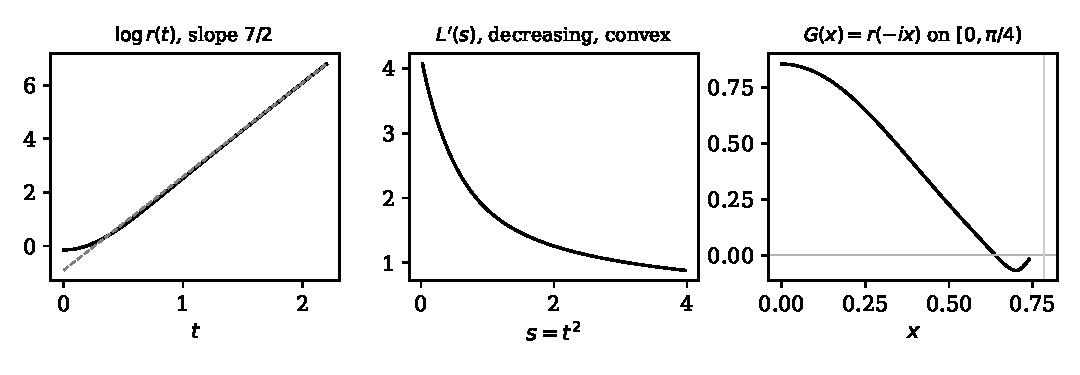
\includegraphics[width=\textwidth]{rzfig/fig_cardon.pdf}
\caption{The Cardon ratio for the random harmonic law $H_{\kappa^*}$. Left: $\log r(t)$ on the real axis, asymptotically linear with slope $\frac72$ (dashed). Centre: $L'(s)$ for $L(s)=\log(r(\sqs)/r(0))$, positive, decreasing and convex as a Stieltjes function must be. Right: the continuation $G(x)=r(-ix)$ on $[0,\pi/4)$, with a simple zero at $x=0.6388$.}
\label{rz:fig:cardon}
\end{figure}

\begin{proposition}\label{rz:prop:cardonnum}
The ratio $r$ satisfies the following necessary conditions for \eqref{rz:eq:cardonrep} (computed).
\begin{enumerate}
\item[(i)] Growth. $r$ is even, $r(0)=0.853936$, and $\log r(t)$ becomes linear with slope approaching $\frac72$: the increments over steps of $0.1$ fall from $0.3534$ to $0.3514$ between $t=1.5$ and $t=2.2$. The slope is explained exactly: $\Phi$ carries the prefactor $e^{9t/2}$, and the saddle point prefactor $\sqrt{s^*/\pi}\approx e^{t}$ of $f_{\kappa^*}$ removes one unit. So $G$ would have exponential type $\frac72$, compatible with order one.
\item[(ii)] Stieltjes signs. With $L(s)=\log r(\sqs)-\log r(0)$, a Laguerre P\'olya $G$ requires $L'(s)=\sum m_k/(s+\alpha_k^2)$, a Stieltjes function. On a grid of $81$ points in $s\in[0,4]$ the difference quotients of $L$ give $L'>0$, $L''<0$ and $L'''>0$ everywhere, and the first order quotients fall from $4.07$ on the first grid interval to $0.94$ on the last.
\item[(iii)] The imaginary axis. The continuation $G(x)=r(-ix)$, computed independently from $\Phi(ix)$ and $f_{\kappa^*}(ix)$, is real, agrees with $r$ at second order ($\log(G(0.1)/G(0))=-0.0423$ against $\log(r(0.1)/r(0))=0.0417$), decreases from $0.8539$, has a simple zero at $\alpha_1=0.6388$, and satisfies the Laguerre inequality $G'^2-GG''\ge2.4>0$ on $[0,0.735]$.
\end{enumerate}
\end{proposition}

Everything visible inside the strip is consistent with $G$ being a Laguerre P\'olya function of exponential type $\frac72$: the single zero $\alpha_1$ accounts for $1/\alpha_1^2=2.45$ of the curvature $\sum m_k/\alpha_k^2\approx4.2$, and a zero density of about $\frac7{2\pi}$ per unit beyond it would account for the linear growth. The decisive question cannot be settled inside the strip.

\begin{proposition}\label{rz:prop:boundary}
If \eqref{rz:eq:cardonrep} holds with $G$ entire, then
\[
f_{\kappa^*}(t)=\Phi(t)/(\Xi(0)G(it)),
\]
so $f_{\kappa^*}$ continues meromorphically exactly as far as $\Phi$ does, and the two share their singular behaviour on the lines $\Im t=\pm\pi/4$, apart from the zeros of $G$. Since $\Phi$ has a natural boundary on these lines, coming from the Jacobi theta function at the edge of its modular domain, $f_{\kappa^*}$ must have the same natural boundary, with singular behaviour proportional to that of $\Phi$ through a factor that continues to an entire function.
\end{proposition}

The first sentence of Proposition~\ref{rz:prop:boundary} is immediate. The second uses the classical fact that the theta function $\omega(x)=\sum_{n\ge1}e^{-\pi n^2x}$ has the line $\Re x=0$ as a natural boundary \cite[Chapter~11, Section~1.4, and Chapter~5, Section~3.2]{Remmert98}, together with $\Phi(t)=4x^{9/4}\omega''(x)+6x^{5/4}\omega'(x)$ at $x=e^{2t}$. Nothing is proved here about whether $f_{\kappa^*}$ has such a boundary; the proposition records what \eqref{rz:eq:cardonrep} would require.

So the random harmonic law fits the P\'olya kernel inside the strip, and the question is the boundary, where the two functions have different origins: $\Phi$ is a modular theta series and $f_{\kappa^*}$ a Rademacher product whose characteristic function has real zeros at $v=(2j+1)\pi(k+\kappa^*)$, increasingly dense. For \eqref{rz:eq:cardonrep} to hold, the Rademacher product would have to reproduce the modular singularities of $\Phi$ up to an entire factor. We see no reason for that, and it suggests that the right Ising system for the P\'olya variable is not the harmonic paramagnet but one whose magnetisation law carries theta function structure.

\subsubsection{The P\'olya variable as the logarithm of a GGC}

Proposition~\ref{rz:prop:boundary} asks for a Lee and Yang system whose magnetisation law carries the modular boundary of $\Phi$. Jacobi's triple product is the first candidate, since it writes a theta function as the characteristic function of a sum of independent two point variables, but these are not Lee and Yang spins (Proposition~\ref{rz:prop:jtp}); the modular structure turns out to live in a multiplicative magnetisation.

\begin{proposition}\label{rz:prop:jtp}
For $0<q<1$ the triple product
\[
\sum_{n\in\mathbb Z}q^{n^2}e^{inv}=\prod_{m\ge1}(1-q^{2m})\bigl(1+2q^{2m-1}\cos v+q^{4m-2}\bigr)
\]
exhibits the discrete Gaussian law $\Pr(J=n)\propto q^{n^2}$ as the law of $\sum_m(B_m-B_m')$ with independent Bernoulli variables of parameter $q^{2m-1}/(1+q^{2m-1})$. Each factor vanishes at $v=\pi\pm i(2m-1)\log(1/q)$, so the characteristic function has no real zeros and the moment generating function has no purely imaginary zeros: the triple product spins are not Lee and Yang spins, and neither is the discrete Gaussian.
\end{proposition}

\begin{proof}
$1+2q^{2m-1}\cos v+q^{4m-2}=(1+q^{2m-1}e^{iv})(1+q^{2m-1}e^{-iv})$, and each factor, normalised, is the characteristic function of a Bernoulli variable or its negative. The zeros are those of $1+q^{2m-1}e^{\pm iv}$.
\end{proof}

So the triple product places the theta function in the field variable, where its zeros lie on horizontal lines rather than on the real axis. For $\Phi$ the theta function enters through the modular variable $e^{2t}$, and the relevant structure is multiplicative. Recall from Section~\ref{ch:clock} the identity of Biane, Pitman and Yor \cite{BPY01}, going back to Williams \cite{Williams90}, which makes this exact.

\begin{theorem}\label{rz:thm:bpy}
Let $S_2=\sum_{k\ge1}\frac{2}{\pi^2k^2}(e_k+e_k')$ with independent standard exponentials $e_k,e_k'$, so that $\E e^{-sS_2}=\bigl(\sqrt{2s}/\sinh\sqrt{2s}\bigr)^2$ and $S_2$ is a GGC with Thorin measure $2\sum_k\delta_{\pi^2k^2/2}$. Then
\[
2\xi(z)=\E\Bigl[\Bigl(\frac{\pi S_2}2\Bigr)^{z/2}\Bigr].
\]
Consequently, with $Y=\frac12\log(\pi S_2/2)$, $2\Xi(\tau)=\E[e^{Y/2}e^{i\tau Y}]$, and the P\'olya variable $X$ is $Y$ tilted by $e^{Y/2}$: $\Phi(t)\,dt=\frac12e^{t/2}\,\Pr(Y\in dt)$.
\end{theorem}

\begin{proof}
This is the identity of \cite[Section~2]{BPY01}; the density of $S_2$ is a theta series by the partial fraction expansion of $(x/\sinh x)^2$ and Poisson summation, and its Mellin transform is $2\xi$.
\end{proof}

We checked the identity exactly at $z=2$ and $z=4$, where $\E S_2=\frac23$ and $\E S_2^2=\frac8{15}$ give $\frac\pi3=2\xi(2)$ and $\frac{2\pi^2}{15}=2\xi(4)$, and numerically at $z=0.8+3i$, where both sides equal $0.8073665638+0.0340962268i$ to ten digits, using $\E V^w=\frac{w}{\Gamma(1-w)}\int_0^\infty s^{-w-1}(1-\E e^{-sV})\,ds$ for positive $V$ and $0<\Re w<1$. Table~\ref{bp:tab:bpy} in Section~\ref{ch:basepoint} checks the identity by simulation at real arguments, and Section~\ref{bp:sec:mellin} there tilts $Y$ to every real basepoint $\sigma$: with no hypothesis, $\xi(\sigma+z)/\xi(\sigma)$ is the moment generating function of $\frac12\log(\frac\pi2S_2)$ under the law of $S_2$ size biased by $S_2^{\sigma/2}$.

Theorem~\ref{rz:thm:bpy} shows where the modular boundary comes from. The P\'olya variable is a tilted logarithm of a GGC whose Thorin atoms lie on the quadratic lattice $\pi^2k^2/2$, and it is the quadratic lattice, through Jacobi's theta function and Poisson summation, that produces the modular natural boundary at $\Im t=\pm\pi/4$: the density of $S_2$ is analytic in $\Re x>0$ with natural boundary on $\Re x=0$, and $x=\frac2\pi e^{2t}$. The Thorin structure thus enters twice: $R$ is the reciprocal moment generating function of the P\'olya variable in $\sqs$, and $S_2$ is a GGC in the usual sense. RH is the statement that every zero of $w\mapsto\E[(\pi S_2/2)^w]$ in the strip $0<\Re w<\frac12$ lies on the line $\Re w=\frac14$.

This suggests a multiplicative Lee and Yang property. We say that a positive random variable $V$ has \emph{Mellin zeros on a line} if $\E V^{w}$, continued, vanishes only on one vertical line. The solved models of the Vere-Jones step have exact multiplicative analogues.

\begin{proposition}\label{rz:prop:multlee}
Let $V=\sum_{k\le n}c_ke_k$ with independent standard exponentials $e_k$ and distinct $c_k>0$. Then $\E V^{u-1}=\Gamma(u)\sum_kA_kc_k^{u}$ with $A_k=c_k^{n-2}/\prod_{j\ne k}(c_k-c_j)$.
\begin{enumerate}
\item[(i)] For $n=2$ the zeros are $u=2\pi i m/\log(c_1/c_2)$, $m\ne0$: all on the line $\Re u=0$. The two exponential sum is a multiplicative solved model.
\item[(ii)] For $n=3$ with $c=(1,\frac14,\frac19)$, a truncation of the quadratic lattice with single atoms, the zeros in $0<\Im u<30$ have real parts $0.488$, $-1.268$, $0.300$, $0.387$, $-1.318$, $0.457$, $0.136$, $-1.129$, $0.500$ (computed): they do not lie on a line.
\end{enumerate}
\end{proposition}

\begin{proof}
The density of $V$ is $\sum_kA_ke^{-x/c_k}$ by partial fractions of $\prod_k(1+c_ks)^{-1}$, and its Mellin transform is the stated exponential polynomial times $\Gamma(u)$. For $n=2$ it is proportional to $c_1^u-c_2^u$. For $n=3$ the zeros are those of $1.5-2.4\cdot4^{-u}+0.9\cdot9^{-u}$, which has none with $|\Re u|\ge8$; the argument principle on $[-8,8]\times[0.01,30]$ counts nine, none lies in $0<\Im u<0.01$, and Newton's method locates them at $0.4881+4.4641i$, $-1.2675+7.6319i$, $0.2997+9.2799i$, $0.3865+13.4112i$, $-1.3178+15.5448i$, $0.4570+18.2547i$, $0.1355+22.4710i$, $-1.1294+23.3902i$ and $0.4998+27.1862i$.
\end{proof}

So the Lee and Yang mechanism survives the passage from additive to multiplicative magnetisations for two components and fails at three, just as a sum of two cosines has real zeros while a generic sum of three need not.
